\chapter{Методы моделирования}

В конце предыдущей главы был сделан вывод о целесообразности построения физической модели метода СЭЛТР для определения возможностей этого метода. При формировании линии в резисте методом СЭЛТР одновременно протекают различные процессы, основными из которых являются:
\begin{itemize}
	\item Рассеяние электронного пучка в резисте и подложке;
	\item Электронно-стимулированные разрывы молекул резиста;
	\item Термическая деполимеризация резиста;
	\item Диффузия продуктов деполимеризации в слое резиста;
	\item Процессы растекания резиста.
\end{itemize}

Отдельно друг от друга эти процессы уже исследовались, и в данной главе приведены существующие подходы к их описанию.


\section{Моделирование рассеяния электронного пучка в веществе}
Поскольку упругие и неупругие процессы, протекающие при рассеянии заряженных частиц в веществе, изучаются практически с начала прошлого века, в настоящее время существует множество подходов к их описанию. При этом, выбрав конкретные модели для процессов упругого и неупругого рассеяния, на основе этих моделей можно реализовать алгоритм моделирования рассеяния электронного пучка в веществе.

\subsection{Модели упругого рассеяния электронов в веществе}
Упругое рассеяние происходит в основном в результате взаимодействия высокоэнергетических электронов с ядрами атомов, частично экранированными их электронами. При этом изменяется направление движения электрона, а его энергия остается практически неизменной. Азимутальный угол рассеяния $\phi$ распределен равномерно в промежутке (0$^\circ$, 360$^\circ$), полярный угол рассеяния $\theta$ распределен в промежутке (0$^\circ$ до 180$^\circ$) со средним значением 5$^\circ$-10$^\circ$.

Основной характеристикой упругого рассеяния электронов на атомах вещества является дифференциальное сечение рассеяния $\frac{d \sigma}{d \Omega}$, определяемое как отношение числа электронов, рассеянных мишенью в элемент телесного угла $d \Omega = d \varphi \sin \theta d \theta$ за единицу времени, к плотности потока электронов. Полное сечение упругого рассеяния определяется как интеграл от дифференциального сечения по полному телесному углу:
\begin{equation} \label{eq:models_1}
	\sigma_\mathrm{el}=2 \pi \int_0^\pi \frac{d \sigma}{d \Omega} \sin \theta d \theta.
\end{equation}

\subsubsection{Формула Резерфорда}
Для определения дифференциального сечения упругого рассеяния электронов на атомах вещества можно воспользоваться формулой Резерфорда~\cite{Dapor_large_book}:
\begin{equation} \label{eq:models_3}
	\frac{d \sigma_\mathrm{R}}{d \Omega}=\frac{Z^2 e^4}{4 E^2(1-\cos \theta+2 \beta)^2},
\end{equation}
где $Z$ -- зарядовое число атомов вещества, $e$ -- заряд электрона, $E$ -- энергия налетающего электрона, $\beta$ -- параметр экранирования. Формула Резерфорда хорошо описывает сечения упругого рассеяния электронов на легких атомах, однако, ее точность снижается с ростом зарядового числа атомов, особенно, в области низких энергий (<1 кэВ)~\cite{Dapor_large_book}.

\subsubsection{Моттовские сечения}
Более точные значения сечений упругого рассеяния (моттовские сечения) могут быть получены за счет решения уравнения Дирака для задачи рассеяния релятивистского электрона в центральном статическом поле атома-мишени~\cite{Czyzewski_mott_cs}. В этом подходе дифференциальное сечение упругого рассеяния задается формулой
\begin{equation}
	\frac{d \sigma_\mathrm{el}}{d \Omega}=|f(\theta)|^2+|g(\theta)|^2,
\end{equation}
где $f(\theta)$ и $g(\theta)$ -- амплитуды рассеяния, соответствующие параллельному и антипараллельному направлению спина электрона относительно его направления движения соответственно и определяемые следующими выражениями:
\begin{equation}
	\begin{aligned}
		&f(\theta)=\frac{1}{2 i K} \sum_{l=0}^{\infty}\left\{(l+1)\left[\exp \left(2 i \delta_l^{-}\right)-1\right]+l\left[\exp \left(2 i \delta_l^{+}\right)-1\right]\right\} P_l(\cos \theta), \\
		&g(\theta)=\frac{1}{2 i K} \sum_{l=0}^{\infty}\left[-\exp \left(2 i \delta_l^{-}\right)+\exp \left(2 i \delta_l^{+}\right)\right] P_l^1(\cos \theta).
	\end{aligned}
\end{equation}
Здесь $k$ -- волновое число налетающего релятивистского электрона, $P_l(\cos \theta)$ и $P_l^1 (\cos \theta)$ -- полиномы Лежандра и присоединенные полиномы Лежандра соответственно, $\delta_l^{\pm}$ -- фазовые сдвиги сферических волн, рассчитываемые по формуле
\begin{equation}
	\tg \left(\delta_l^{\pm}\right)=\frac{K j_{l+1}(K r)-j_l(K r)\left[(W+1) \tg \phi_l^{\pm}+\left(1+l+k^{\pm}\right) / r\right]}{K n_{l+1}(K r)-n_l(K r)\left[(W+1) \tg \phi_l^{\pm}+\left(1+l+k^{\pm}\right) / r\right]},
\end{equation}
где $K^2 = W^2 - 1$ , $W$ -- полная энергия электрона в единицах $mc^2$, $r$ -- расстояние до рассеивающего центра в единицах $h/2 \pi mc$. 
Индексы ``+'' и ``0'' обозначают параллельное и антипараллельное направление спина, соответственно:
\begin{equation}
	\begin{aligned}
		&+: k^{+}=-l-1, \quad & j=l+1 / 2, \\
		&-: k^{-}=l, \quad & j=l-1 / 2 .
	\end{aligned}
\end{equation}
При этом $\phi_l^\pm$ -- предел функции $\phi_l^\pm (r)$ (при $r \rightarrow \infty$), которая находится путем численного интегрирования уравнения Дирака:
\begin{equation}
	\frac{d \phi_l^{\pm}(r)}{d r}=\frac{k^{\pm}}{r} \sin \left[2 \phi_l^{\pm}(r)\right]-\cos \left[2 \phi_l^{\pm}(r)\right]+W-V(r),
\end{equation}
где $V(r)$ -- рассеивающий потенциал.


\subsection{Модели квазиупругого рассеяния электронов в веществе}
\subsubsection{Модель электрон-фононного рассеяния}
За счет теплового движения атомы кристаллических тел колеблются вблизи своих положений равновесия. С такими колебаниями связывается наличие фононов в кристаллической решетке, и их число может изменяться за счет взаимодействия налетающего электрона с оптическими модами колебаний решетки~\cite{Fronlich_phonons, Llacer_phonons}. Энергия фононов не превышает значения $\kB T_\mathrm{D}$, где $\kB$ -- постоянная Больцмана и $T_\mathrm{D}$ -- температура Дебая. Для большинства твердых тел величина $\kB T_\mathrm{D}$ составляет менее 0.1 эВ, и учет потерь энергии налетающего электрона за счет генерации фононов становится целесообразен при энергиях электрона порядка 1~эВ~\cite{Ganachaud_phonons_polarons}.

Согласно существующим работам~\cite{Fronlich_phonons, Llacer_phonons}, обратная длина свободного пробега при электрон-фононном рассеянии может быть выражена формулой
\begin{equation} \label{eq:phonons}
	\lambda_{\mathrm{ph}}^{-1}=\frac{1}{a_0} \frac{\varepsilon_0-\varepsilon_{\infty}}{\varepsilon_0 \varepsilon_{\infty}} \frac{\hbar \omega}{E} \frac{n(T)+1}{2} \ln \left[\frac{1+\sqrt{1-\hbar \omega / E}}{1-\sqrt{1-\hbar \omega / E}}\right],
\end{equation}
где $E$ -- энергия налетающего электрона, $\hbar \omega$ -- его потери энергии (порядка 0.01–0.1 эВ), $\varepsilon_0$ -- статическая диэлектрическая проницаемость, $\varepsilon_\infty$ -- высокочастотная диэлектрическая проницаемость, $a_0$ -- боровский радиус и $n(T)$ -- число заполнения:
\begin{equation}
	n(T)=\frac{1}{e^{\hbar \omega / kB T}-1},
\end{equation}
где $\kB$ -- постоянная Больцмана. Было установлено, что для ПММА величина $\hbar \omega$ может быть принята равной 0.1 эВ~\cite{Fronlich_phonons, Llacer_phonons}, что вкупе с формулой~\ref{eq:phonons} предоставляет все необходимое для моделирования электрон-фононного взаимодействия.


\subsubsection{Модель электрон-поляронного рассеяния}
Электроны, медленно движущиеся в диэлектриках, приводят к появлению поляризационного поля, которое оказывает на них стабилизирующее воздействие. Такой процесс описывается как генерация квазичастицы – полярона, состоящего из электрона и поляризационного облака вокруг него. Было установлено, что энергетическая зависимость обратной длины свободного пробега электрона при таком взаимодействии может быть описана экспоненциальной функцией~\cite{Ganachaud_phonons_polarons}:
\begin{equation}
	\lambda_\mathrm{pol}^{-1}=C e^{-\gamma E}.
\end{equation}
Параметры $C$ и $\gamma$ определяются косвенным методом (например, путем анализа различных распределений для вторичных электронов~\cite{Ciappa_2010, Dapor2011}). При этом считается, что при генерации полярона налетающий электрон полностью останавливается ($\hbar \omega = E$). Было установлено, что для ПММА параметры $C$ и $\gamma$ могут быть приняты равными 0.1 нм$^\text{-1}$ и 0.15 эВ$^\text{-1}$ соответственно~\cite{Dapor_large_book}. Следует отметить, что в силу фиксированных потерь энергии как при электрон-фононном, так и при электрон-поляронном рассеянии допустимо непосредственное использование обратной длины свободного пробега (без предварительного вычисления дифференциальной обратной длины свободного пробега).


\subsection{Модели неупругого рассеяния электронов в веществе}
Квазиупругие и неупругие процессы включают в себя все процессы взаимодействия между налетающим электроном и веществом мишени, в которых электрон теряет свою энергию. При этом также происходит изменение направления движения электрона, и полярный угол рассеяния $\theta$ задается выражением~\cite{Ciappa_2010}
\begin{equation}
	\sin ^2 \theta=\frac{\hbar \omega}{E},
\end{equation}
где $E$ -- энергия электрона до акта рассеяния, $\hbar \omega$ -- потери энергии. В моделях неупругого рассеяния часто рассматривается взаимодействие налетающего электрона с веществом мишени в целом, и для описания такого взаимодействия используется обратная длина свободного пробега $\lambda_\mathrm{inel}^{-1}(E)$, связанная с сечением неупругого рассеяния формулой
\begin{equation}
	\lambda_{\text{inel}}^{-1}(E) = n \sigma(E),
\end{equation}
где $n$ -- концентрация рассеивающих центров в веществе.


\subsubsection{Модель непрерывных потерь энергии}
Исторически первые подходы к описанию потерь энергии электрона в веществе основывались на формуле Бете~\cite{Bethe}:
\begin{equation}
	-\left(\frac{d E}{d s}\right)_{\text {Bethe }}=2 \pi e^4 N_\mathrm{A} \frac{\rho}{Z} \frac{1}{E} \ln \left(\frac{1.66 E}{J}\right),
\end{equation}
где $N_\mathrm{A}$ -- число Авогадро, $\rho$ -- плотность вещества, $Z$ -- порядковый номер атомов вещества, $e$ и $E$ -- заряд и энергия движущегося в веществе электрона соответственно. Средний потенциал ионизации $J$ определяется экспериментально или вычисляется на основе порядкового номера атомов вещества~\cite{Dapor_large_book}:
\begin{equation}
	\frac{J}{Z} = 9.76 + 58.8 Z^{-1.19}.
\end{equation}
Формула Бете с высокой точностью описывает потери энергии в области высоких энергий налетающего электрона ($E \gg J$). Однако, при приближении энергии налетающего электрона к среднему потенциалу ионизации точность формулы снижается, а в области $E < J$ потери энергии, рассчитываемые по ней, становятся отрицательными. Существуют модификации формулы Бете, позволяющие использовать ее в области низких энергий, в которых потери энергии при $E \rightarrow 0$ описываются степенной функцией~\cite{Bethe_corrected}:
\begin{equation}
	-\frac{dE}{ds} \propto \frac{1}{\sqrt{E}}.
\end{equation}
В таком виде формула Бете может быть использована, например, для оценки количества обратно отраженных и вторичных электронов, что дает правдоподобные результаты~\cite{Bethe_corr_2ndary_e}. Однако, неограниченный рост потерь энергии при $E \rightarrow 0$ противоречит эмпирическим данным, согласно которым при уменьшении энергии налетающего электрона его потери энергии достигают максимума при энергии в несколько сотен электрон вольт, затем стремятся к нулю~\cite{Shimizu_Review}.


\subsubsection{Модель дискретных потерь энергии}
В современных моделях неупругого рассеяния потери энергии электрона в веществе сводятся к дискретным процессам. В них, аналогично случаю с упругим рассеянием, вводится дифференциальная обратная длина свободного пробега $\frac{d \lambda_\mathrm{inel}^{-1}}{d \hbar \omega}(E, \hbar \omega)$, позволяющая определить обратную длину свободного пробега по формуле~\cite{Dapor_large_book}
\begin{equation}
	\lambda_\mathrm{inel}^{-1}(E)=\int_0^{E / 2} \frac{d \lambda_{\text {inel }}^{-1}(E, \hbar \omega)}{d \hbar \omega} d \hbar \omega,
\end{equation}
а также потери энергии электрона на единицу длины пути $\frac{dE}{ds}$ по формуле
\begin{equation}
	\frac{dE}{ds}(E) = \int_0^{E / 2} \frac{d \lambda_\mathrm{inel}^{-1}(E, \hbar \omega)}{d \hbar \omega} \hbar \omega d \hbar \omega.
\end{equation}
Потери энергии $\hbar \omega$ при неупругом рассеянии также определяются на основе функции $\frac{d \lambda_\mathrm{inel}^{-1}}{d \hbar \omega}$  методом Монте-Карло~\cite{Ciappa_2010}.

Наиболее распространенный подход к определению дифференциальной обратной длины свободного пробега основан на использовании функции потерь энергии (Energy Loss Function, ELF)~\cite{Dapor_large_book}:
\begin{equation}
	\operatorname{ELF}(q, \omega) \equiv \operatorname{Im}\left[\frac{-1}{\varepsilon(q, \omega)}\right].
\end{equation}
Здесь $\varepsilon(q, \omega)$ -- комплексная диэлектрическая функция, $\vec{q}$ и $\hbar \omega$ -- передаваемые среде импульс и энергия соответственно. При известной функции потерь энергии дифференциальная обратная длина свободного пробега может быть найдена по формуле
\begin{equation}
	\frac{d \lambda_{\text {inel }}^{-1}}{d \hbar \omega}=\frac{1}{\pi E a_0} \int_{k_{-}}^{k_{+}} \operatorname{Im}\left[\frac{-1}{\varepsilon(q, \omega)}\right] \frac{d q}{q},
\end{equation}
где
\begin{equation}
	q_{\pm}=\frac{\sqrt{2 m}}{\hbar}(\sqrt{E} \pm \sqrt{E-\hbar \omega}),
\end{equation}
$E$ -- энергия налетающего электрона, $m$ -- масса электрона и $a_0$ -- боровский радиус.

Поскольку функция $\varepsilon(q, \omega)$ может быть найдена из первых принципов только в некоторых идеализированных случаях~\cite{Ritchie_ELF}, часто используется подход на основе оптической функции потерь энергии (Optical Energy Loss Function, OELF), получаемой в пределе $q \rightarrow 0$:
\begin{equation}
	\operatorname{OELF}(\omega) \equiv E L F(0, \omega)=\operatorname{Im}\left[\frac{-1}{\varepsilon(0, \omega)}\right].
\end{equation}
Оптическая функция потерь энергии может быть рассчитана на основе значений коэффициентов преломления ($n$) и поглощения ($k$)~\cite{Dapor_2015_oscillators} (рисунок~\ref{fig:OLF} a)):
\begin{equation}
	\operatorname{Im}\left[\frac{-1}{\varepsilon(0, \omega)}\right]=\frac{2 n k}{\left(n^2+k^2\right)^2}.
\end{equation}
Коэффициенты $n$ и $k$ табулированы для многих веществ в области низких энергий (примерно до 2~кэВ)~\cite{Palik}, для более высоких энергий они могут быть определены из компонент атомных факторов рассеяния $f = f_1 + i f_2$ (для молекулярных веществ)~\cite{Henke_photoabs}:
\begin{equation}
	\begin{aligned}
		&n=1-\frac{e^2}{2 \pi m c^2} \lambda^2 N \sum_p x_p f_{1 p}, \\
		&k=\frac{e}{2 \pi m c^2} \lambda^2 N \sum_p x_p f_{2 p}.
	\end{aligned}
\end{equation}
Здесь $N$ -- концентрация молекул, содержащих $x_p$ атомов каждого вида, $\lambda$ -- длина волны фотона. Для атомарных веществ оптическая функция потерь энергии может быть найдена непосредственно по формуле
\begin{equation}
	\operatorname{Im}\left[\frac{-1}{\varepsilon(0, \omega)}\right]=\frac{n_\mathrm{c} c \sigma_\mathrm{phot}}{\omega},
\end{equation}
где $n_\mathrm{c}$ -- концентрация остовных электронов, $\sigma_\mathrm{phot}$ --  сечение фотоионизации~\cite{Biggs_cs}. При известной оптической функции потерь энергии поведение функция потерь энергии в области $q > 0$ учитывается с помощью одного из подходов, описанных ниже.


\paragraph{Аппроксимация функции потерь энергии эмпирической функцией} \mbox{} \\
\indent Наиболее простым является подход, в котором поведение функции потерь энергии в области $q > 0$ учитывается за счет использования эмпирических функций $L(x)$ и $S(x)$, что позволяет непосредственно рассчитать обратную длину свободного пробега~\cite{Ashley_LxSx}
\begin{equation}
	\begin{aligned}
		&\lambda^{-1}(E)=\frac{m e^2}{2 \pi \hbar^2 E} \int_0^{W_{\max }} \operatorname{Im}\left[\frac{-1}{\varepsilon(0, \omega)}\right] L\left(\frac{\hbar \omega}{E}\right) d \hbar \omega, \\
		&L(x)=(1-x) \ln \frac{4}{x}-\frac{7}{4} x+x^{3 / 2}-\frac{33}{32} x^2,
	\end{aligned}
\end{equation}
а также потери энергии на единицу длины пути
\begin{equation}
	\begin{aligned}
		&\lambda^{-1}(E)=\frac{m e^2}{2 \pi \hbar^2 E} \int_0^{W_{\max }} \operatorname{Im}\left[\frac{-1}{\varepsilon(0, \omega)}\right] L\left(\frac{\hbar \omega}{E}\right) d \hbar \omega, \\
		&L(x)=(1-x) \ln \frac{4}{x}-\frac{7}{4} x+x^{3 / 2}-\frac{33}{32} x^2.
	\end{aligned}
\end{equation}



\paragraph{Аппроксимация функции потерь энергии суммой осцилляторов Друде} \mbox{} \\
\indent В данном подходе оптическая функция потерь энергии приближается суммой осцилляторов Друде~\cite{Ritchie_Drude} (рисунок~\ref{fig:OLF} б)):
\begin{equation}
	\operatorname{Im}\left[\frac{-1}{\varepsilon(0, \omega)}\right]=\sum_i \frac{A_i \Gamma_i \hbar \omega}{\left[E_i^2-(\hbar \omega)^2\right]^2+\left(\Gamma_i \hbar \omega\right)^2}.
\end{equation}
Параметры отдельных осцилляторов $E_i$, $\Gamma_i$ и $A_i$ определяются путем аппроксимации оптической функции потерь энергии~\cite{Dapor_2015_oscillators}, а продолжение оптической функции потерь энергии в область осуществляется за счет использования квадратичного закон дисперсии:
\begin{equation}
	E_i(q)=E_i+\frac{\hbar^2 q^2}{2 m},
\end{equation}
что в дальнейшем позволяет получить функцию потерь энергии:
\begin{equation}
	\operatorname{Im}\left[\frac{-1}{\varepsilon(q, \omega)}\right]=\sum_i \frac{A_i \Gamma_i \hbar \omega}{\left[\left(E_i+\frac{\hbar^2 q^2}{2 m}\right)^2-(\hbar \omega)^2\right]^2+\left(\Gamma_i \hbar \omega\right)^2}.
\end{equation}

\begin{figure}[t]
	\begin{minipage}{0.5\textwidth}
		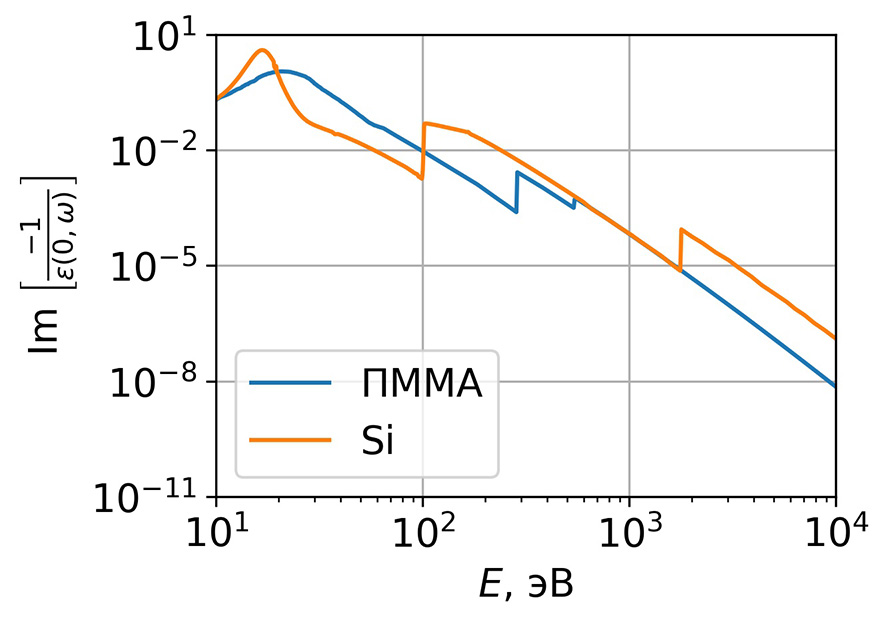
\includegraphics[width=\linewidth]{OLF/PMMA_Si_OLF_shrink_200} \\
		\vspace{-12.5em} \\ \text{\hspace{0em} a}) \\ \vspace{12.5em}
	\end{minipage}
	\begin{minipage}{0.5\textwidth}
		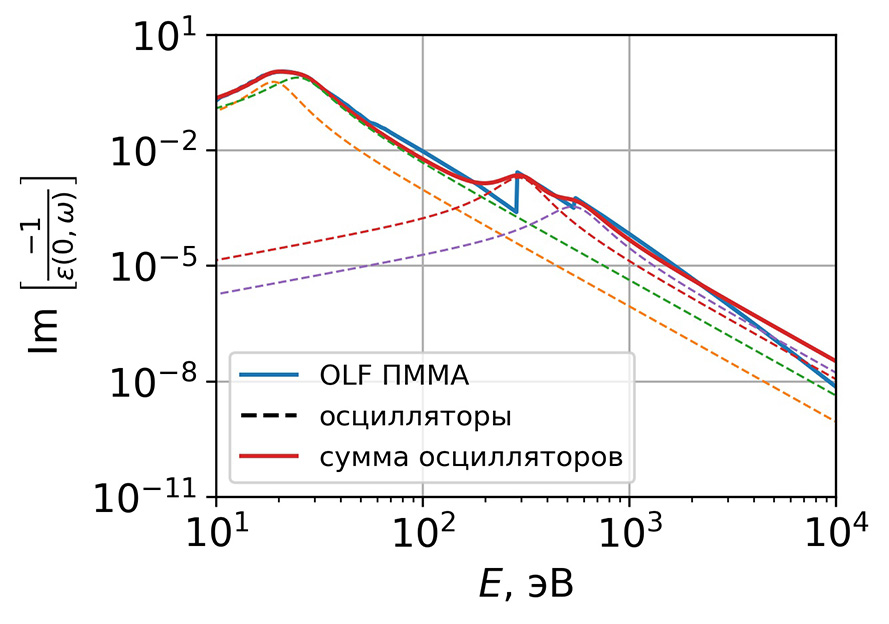
\includegraphics[width=\linewidth]{OLF/OLF_PMMA_fit_200} \\
		\vspace{-12.5em} \\ \text{\hspace{-0.1em} б}) \\ \vspace{12.5em}
	\end{minipage}
	\vspace{-3.5em}
	\caption{а) Оптическая функции потерь энергии, рассчитанная для ПММА и Si~\cite{Palik, Ritchie_ELF}, б) оптическая функция потерь энергии ПММА, приближенная суммой осцилляторов Друде~\cite{Dapor_2015_oscillators}.}
	\label{fig:OLF}
\end{figure}


\paragraph{Диэлектрическая функция Мермина} \mbox{} \\
\indent Наиболее точным подходом к определению функции потерь энергии для органических полимеров является подход на основе модели Мермина~\cite{Mermin}. В его основе лежит диэлектрическая функция Мермина для столкновительной плазмы:
\begin{equation}
	\varepsilon_\mathrm{M}(q, \omega)=1+\frac{(1+i \gamma / \omega)\left[\varepsilon_\mathrm{L}(q, \omega+i \gamma)-1\right]}{1+(i \gamma / \omega)\left[\varepsilon_\mathrm{L}(q, \omega+i \gamma)-1\right] /\left[\varepsilon_\mathrm{L}(q, 0)-1\right]},
\end{equation}
где $\gamma$ -- постоянная затухания, $\varepsilon_\mathrm{L}(q, \omega)$ -- диэлектрическая функция Линдхарда~\cite{Lindhard}:
\begin{equation}
	\varepsilon_\mathrm{L}(q, \omega)=1+\frac{\chi^2}{z^2}\left[f_1(u, z)+i f_2(u, z)\right].
\end{equation}
Здесь $u=\omega /\left(q v_\mathrm{F}\right)$, $z=q /\left( 2 q_\mathrm{F} \right)$ и $\chi^2=e^2 / \left( \pi \hbar v_\mathrm{F} \right)$, где $v_\mathrm{F}$
-- скорость Ферми валентных электронов вещества, $q_F=m v_\mathrm{F} / \hbar$. При этом функции $f_1(u, z)$ и $f_2(u, z)$ определяются формулами
\begin{equation}
	\begin{aligned}
		f_1(u, z) &=\frac{1}{2}+\frac{1}{8 z}[g(z-u)+g(z+u)], \\
		f_2(u, z) &= \begin{cases}\frac{\pi}{2} u, & z+u<1 \\
			\frac{\pi}{8 z}\left[1-(z-u)^2\right], & |z-u|<1<z+u \\
			0, & |z-u|>1\end{cases},
	\end{aligned}
\end{equation}
где
\begin{equation}
	g(x)=\left(1-x^2\right) \ln \left|\frac{1+x}{1-x}\right|.
\end{equation}

Как и в предыдущем случае, функция потерь энергии вещества описывается суммой функций потерь энергии, соответствующих отдельным осцилляторам, и ее вычисление производится в два этапа. Сначала оптическая функция потерь энергии вещества аппроксимируется суммой функций потерь энергии Мермина (осцилляторов Мермина) для $q=0$:
\begin{equation}
	\operatorname{Im}\left[\frac{-1}{\varepsilon(0, \omega)}\right]=\sum_i A_i \operatorname{Im}\left[\frac{-1}{\varepsilon_\mathrm{M}\left(\omega_i, \gamma_i, q=0, \omega\right)}\right],
\end{equation}
что позволяет получить параметры $A_i$, $\omega_i$ и $\gamma_i$ отдельных осцилляторов~\cite{DeVera_MELF_params}. Параметр $\omega_i$ определяет частоту каждого из осцилляторов, что позволяет определить значение параметра $v_\mathrm{F}$, входящего в величины $u$, $z$ и $\chi$, используемые в диэлектрической функции Линдхарда:
\begin{equation}
	\begin{aligned}
		&\omega_i=\sqrt{\frac{4 \pi n_i e^2}{m}} \Rightarrow n_i=\frac{\omega_i^2 m}{4 \pi e^2}, \\
		&v_{\mathrm{F}_i}=\frac{\hbar}{m}\left(3 \pi^2 n_i\right)^{1/3},
	\end{aligned}
\end{equation}
где $n_i$ -- концентрация электронов, соответствующая осциллятору с индексом $i$, $m$ -- масса электрона. Далее на основе параметров $A_i$, $\omega_i$ и $\gamma_i$ определяется функция потерь энергии:
\begin{equation}
	\operatorname{Im}\left[\frac{-1}{\varepsilon(q, \omega)}\right]=\sum_i A_i \operatorname{Im}\left[\frac{-1}{\varepsilon_\mathrm{M}\left(\omega_i, \gamma_i, q, \omega\right)}\right],
\end{equation}
что позволяет вычислить дифференциальную обратную длину свободного пробега.

\subsection{Моделирование на основе кинетической теории транспорта}
Моделирование на основе кинетической теории транспорта заключается в решении кинетического уравнения Больцмана, описывающего распространение электронов в структуре. Этот метод успешно применяется для моделирования рассеяния электронного пучка в планарных структурах, состоящих из небольшого количества слоев~\cite{Stepanova_2006, Stepanova_2010}. Для задач с более сложной геометрией необходимо введение дополнительных граничных условий, что значительно усложняет расчет.


\paragraph{Определение распределения электронов по глубине} \mbox{} \\
\indent В большинстве случаев для упрощения расчетов, рассматривается точечный (в плоскости $XY$) пучок электронов, направленный под прямым углом к поверхности (вдоль оси $Z$). Распространение электронов в веществе по глубине может быть описано функцией распределения $f(z, E, \cos \theta_v)$, где $z$, $E$ -- глубина проникновения электрона в образец и его энергия, $\cos \theta_v$ -- угол между скоростью электрона и осью $z$. В этом случае уравнение Больцмана принимает вид~\cite{ME_rev_60}:
\begin{equation} \label{eq:Boltzman_1}
	\frac{d E}{d s} \frac{\partial f}{\partial E}+\cos \theta_v \frac{\partial f}{\partial z}=\frac{1}{\Lambda} \int w(\cos \gamma)\left[f\left(\cos \theta_{v^{\prime}}\right)-f\left(\cos \theta_v\right)\right] d \Omega_\gamma,
\end{equation}
где $\frac{dE}{ds}$ -- потери энергии на единицу длины пути, $\Lambda$ -- длина свободного пробега при упругом рассеянии, $v$ и $v^{\prime}$ -- скорости до и после рассеяния, соответственно, $w(\cos \gamma)$ -- нормированное дифференциальное сечение упругого рассеяния на угол $\gamma$:
\begin{equation} \label{eq:Boltzman_2}
	w(\cos \gamma)=\frac{1}{\sigma_{\mathrm{el}}} \frac{d \sigma}{d \Omega_\gamma}.
\end{equation}
Уравнение \ref{eq:Boltzman_1} может быть решено в диффузионном приближении~\cite{ME_rev_61}, применимом в диапазоне энергий, характерных для электронно-лучевой литографии. Для этого функция распределения электронов раскладывается в ряд по полиномам Лежандра $P(\cos \theta)$:
\begin{equation} \label{eq:Boltzman_3}
	f\left(z, E, \cos \theta_v\right)=\sum_0^{\infty} C_n(z, E) P_n\left(\cos \theta_n\right).
\end{equation}
Подстановка \ref{eq:Boltzman_3} в \ref{eq:Boltzman_1} приводит к дифференциальной разностной схеме для коэффициентов $C_n$:
\begin{equation} \label{eq:Boltzman_4}
	\left(\frac{d E}{d s}\right) \frac{\partial C_n}{\partial E}+\frac{n}{2 n-1} \frac{\partial C_{n-1}}{\partial z}+\frac{n+1}{2 n+3} \frac{\partial C_{n+1}}{\partial z}=-\frac{1}{\lambda_n} C_n,
\end{equation}
где
\begin{equation} \label{eq:Boltzman_5}
	\frac{1}{\lambda_n}=\frac{1}{\Lambda} \int\left[1-P_n(\cos \gamma)\right] W(\cos \gamma) d \Omega_\gamma.
\end{equation}
Коэффициенты $C_0$ и $C_1$ пропорциональны плотности вероятности и проекции плотности потока вероятности на ось $z$, соответственно:
\begin{equation} \label{eq:Boltzman_6}
	\begin{gathered}
		\rho(z, E)=\int f\left(z, E, \cos \theta_v\right) d \Omega_v=4 \pi C_0(z, E), \\
		J_z(z, E)=\int v \cos \theta_v f\left(z, E, \cos \theta_v\right) d \Omega_v=\frac{4 \pi}{3} v C_1(z, E).
	\end{gathered}
\end{equation}
Точное решение \ref{eq:Boltzman_1} возможно при отбрасывании в  коэффициентов $C_n$ с \break $n>1$, соответствующих турбулентному движению. При этом уравнение~\ref{eq:Boltzman_4} принимает вид уравнения диффузии:
\begin{equation} \label{eq:Boltzman_7}
	\frac{\partial}{\partial E} \rho(z, E)=a(E) \frac{\partial^2}{\partial z^2} \rho(z, E), a(E)=\left(\frac{d E}{d s}\right)^{-1} \frac{\lambda_1}{3}.
\end{equation}
Его решение:
\begin{equation} \label{eq:Boltzman_8}
	\rho(z, E)=\frac{1}{\sqrt{\pi} \sigma(E)} \exp \left(-\frac{z^2}{4 \sigma^2(E)}\right)\left\{1-\frac{\sqrt{\pi} \sigma(E)}{\Delta \lambda_1\left(E_0\right)} \exp \left(\zeta^2\right) \operatorname{erfc}\left(\zeta^2\right)\right\},
\end{equation}
где
\begin{equation} \label{eq:Boltzman_9}
	\zeta = \frac{z}{2 \sigma(E)}+\frac{\sigma(E)}{\Delta \lambda_1\left(E_0\right)}, \quad \sigma^2=\int a(E) d E, \quad \Delta=0.71.
\end{equation}
Для описания функции распределения электронов в системе, состоящей из нескольких слоев, решение для предыдущего слоя используется как граничное условие для уравнения диффузии в новом слое.


\paragraph{Определение латерального распределения электронов} \mbox{} \\
\indent Латеральное распределение электронов описывается функцией плотности вероятности $\rho(r, z, E)$, определяющей вероятность нахождения электрона с энергией $E$ в кольце радиуса $r$, имеющем объем $2 \pi r dr dz$ и расположенном параллельно поверхности резиста на глубине $z$. Для определения продольного распределения электронов необходимо решение уравнения Больцмана в более общем виде, чем \ref{eq:Boltzman_1}~\cite{ME_rev_63}, и при этом отдельно учитывается вклад от электронов, рассеянных на малые углы (индекс ``$\mathrm{f}$''), обратно рассеянных электронов (индексы ``$\mathrm{bd}$'' и ``$\mathrm{bs}$'') и вторичных электронов (индекс ``$\mathrm{s}$'')~\cite{ME_rev_64}:
\begin{equation} \label{eq:Boltzman_10}
	\rho(r, z, E)=\rho(z, E)\left[\rho_\mathrm{f}(r \mid z, E)+\rho_\mathrm{bd}(r \mid z, E)\right]+\rho_\mathrm{bs}(r, z, E)+\rho_\mathrm{s}(r, z, E).
\end{equation}
Здесь выражения вида $\rho(r|z,E)$ означают плотность вероятности при известных значениях $z$ и $E$. Слагаемое $\rho_\mathrm{f}(r|z,E)$ описывает продольное уширение пучка за счет небольшого количества актов рассеяния первичных электронов на малые углы в слое резиста:
\begin{equation} \label{eq:Boltzman_11}
	\rho_f(r \mid z, E)=\frac{3 \lambda_1}{2 \pi z^3} \exp \left(-\frac{3 \lambda_1 r^2}{2 z^3}\right),
\end{equation}
где $\lambda_1$ определяется из соотношения \ref{eq:Boltzman_5}.

Обратное рассеяние электронов происходит за счет рассеяния на большие углы вблизи границы резиста с подложкой ($\rho_\mathrm{bs}$), либо за счет диффузии электронов в структуре ($\rho_\mathrm{bd}$):
\begin{equation} \label{eq:Boltzman_12}
	\begin{gathered}
		\rho_\mathrm{bs}(r, z, E)=\frac{1}{\pi} \int_z^{z_\mathrm{d}} \beta(1+\beta) \rho\left(z^{\prime}, E\right) \frac{z^{\prime}-z}{R} \frac{d z^{\prime} / \Lambda}{\left[(1+\beta) R+z^{\prime}-z\right]^2}, \\
		\rho_\mathrm{bd}(r \mid z, E)=\frac{A^2}{3} \int_{z_\mathrm{d}}^{z_\mathrm{max}}\left(\frac{1}{4 \pi \sigma_\mathrm{b}^2}\right)^{3 / 2} \exp \left(-\frac{R^2}{4 \sigma_\mathrm{b}^2}\right) \frac{z^{\prime}-z}{z_{\max }-z_\mathrm{d}} d z^{\prime},\\
		R=\sqrt{r^2+\left(z-z^{\prime}\right)^2}, \\ \sigma_\mathrm{b}^2=\int_{E\left(z^{\prime}\right)}^{E(z)} a\left(E^{\prime}\right) d E^{\prime},
	\end{gathered}
\end{equation}
где $\beta$ -- параметр экранирования в формуле Резерфорда для дифференциального сечения упругого рассеяния, $\Lambda$ -- длина свободного пробега при упругом рассеянии, $a(E)$ -- коэффициент диффузии в уравнении~\ref{eq:Boltzman_7}, $E(z)$ , $E(z^\prime)$ -- средние энергии электрона, получаемые за счет интегрировании функции $Ef(z, E, \cos \theta_v )$. Параметр $z_\mathrm{d}$ выражает максимальную глубину проникновения электронов, рассеивающихся на большие углы вблизи границы резиста с подложкой, и его значение подбирается на основе моделирования методом Монте-Карло. Значения параметров $z_\mathrm{max}$ и $A$, определяющих максимальную глубину, на которой могут находиться обратно отраженные электроны, и коэффициент обратного отражения электронов соответственно, также выбираются исходя из результатов моделирования методом Монте-Карло. Например, для слоя полиметилметакрилата (ПММА) толщиной 0.5 мкм на кремниевой подложке используются следующие значения этих параметров: $z_\mathrm{d}$ = 0.83 мкм, $z_\mathrm{max}$ = 8.5 мкм, $A$ = 0.19.

Уширение пучка за счет генерации вторичных электронов описывается функцией плотности вероятности для вторичных электронов:
\begin{equation} \label{eq:Boltzman_13_0}
	\begin{split}
		\rho_\mathrm{s}(r, z, E) = \int_{2 E}^{E_0} d E^{\prime} & p_\mathrm{inel} \left(E^{\prime}\right) \Phi\left(E, E^{\prime}\right) \times \\
		& \times \int d^3 \vec{r}^{\prime} \frac{1}{8 \pi S^3(E)} \exp \left(\frac{-\left|\vec{r}-\vec{r}^{\prime}\right|}{S(E)}\right) \rho\left(r^{\prime}, z, E^{\prime}\right).
	\end{split}
\end{equation}
Здесь $E_0$ -- начальная энергия электронов, $p_\mathrm{inel}$ -- вероятность неупругого рассеяния с генерацией вторичного электрона, определяемая на основе сечений упругого и неупругого рассеяния ($\sigma_\mathrm{el}(E)$ и $\sigma_\mathrm{inel}(E)$, соответственно):
\begin{equation} \label{eq:Boltzman_13}
	p_\mathrm{inel}(E) = \frac{\sigma_\mathrm{inel}}{\sigma_\mathrm{el}+\sigma_\mathrm{inel}}.
\end{equation}
Функция $\Phi\left(E, E^{\prime}\right)$ представляет собою дифференциальное сечение неупругого рассеяния, нормированное на полное сечение неупругого рассеяния, $S(E)$ -- максимальная глубина проникновения электронов, выражаемая через потери энергии на единицу пути:
\begin{equation} \label{eq:Boltzman_14}
	S(E)=\int_{E_0}^{E_{\min }} d E\left(\frac{d E}{d s}\right)^{-1}.
\end{equation}

Одним из наиболее важных результатов моделирования в этом случае является распределение энергии, выделившейся в резисте при экспонировании. Плотность выделившейся энергии в пересчете на один первичный электрон может быть получена за счет интегрирования произведения плотности вероятности и функции потерь энергии~\cite{ME_rev_64}.


\subsection{Моделирование методом Монте-Карло}
В отличие от моделирования на основе кинетической теории транспорта, при моделировании методом Монте-Карло траектория каждого первичного или вторичного электрона рассчитывается отдельно. Параметры траектории и потери энергии электрона определяются на основе дифференциальных сечений процессов упругого и неупругого рассеяния с использованием случайных чисел, равномерно распределенных на промежутке [0, 1). Данный метод требует больших вычислительных мощностей, чем вышеописанный метод моделирования на основе кинетической теории транспорта, но при этом его сложность практически не зависит от формы структуры и количества входящих в нее материалов. Также, в отличие от моделирования на основе кинетической теории транспорта, моделирование рассеяния электронного пучка в веществе методом Монте-Карло позволяет воспроизвести стохастический характер процессов рассеяния.

\paragraph{Определение длины пробега электрона} \mbox{} \\
\indent Полные сечения процессов упругого и неупругого рассеяния электронов в веществе вычисляются путем интегрирования дифференциальных сечений соответствующих процессов:
\begin{equation} \label{eq:MC_1}
	\sigma_\mathrm{el/inel}(E) = \int_Q \frac{d \sigma_\mathrm{el/inel}(E, q)}{dq} dq,
\end{equation}
где индекс ``$\mathrm{el/inel}$'' обозначает тип рассеяния -- упругое рассеяние или неупругое, соответственно. Дифференциальные сечения рассеяния зависят как от энергии налетающего электрона, так и от второй переменной, которая здесь называется $q$. Для упругого рассеяния это полярный угол рассеяния $\theta$, для неупругого -- энергия $\Delta E$, передаваемая налетающим электроном среде. Интегрирование в формуле \ref{eq:MC_1} производится по области всех возможных значений $q$. Далее длина свободного пробега электрона в веществе определяется по формуле
\begin{equation} \label{eq:MC_4}
	\lambda^{-1}(E) = \lambda_\mathrm{el}^{-1}(E)+\lambda_\mathrm{inel}^{-1}(E),
\end{equation}
где
\begin{equation} \label{eq:MC_3}
	\lambda_\mathrm{el/inel}(E)=\left(n \sigma_\mathrm{el/inel}(E)\right)^{-1},
\end{equation}
$n$ -- концентрация рассеивающих центров в веществе.

Вероятность того, что на промежутке пути длиной $s$ не произойдет рассеяния, равна~\cite{ME_rev_49}
\begin{equation} \label{eq:MC_5}
	p(s) = \lambda(E)^{-1} \exp \left(-\frac{s}{\lambda(E)}\right).
\end{equation}
Длина пробега электрона может быть определена по формуле
\begin{equation} \label{eq:MC_6}
	s = -\lambda(E) \ln \left(\xi_1\right),
\end{equation}
где $\xi_1$ случайное число из промежутка [0, 1). Если пробег электрона начинается и заканчивается в слоях, состоящих из разного вещества (например, моделирование производится для системы из $m$ слоев с толщинами $s_1$, $s_2$, ..., $s_m$ и длинами свободного пробега электронов $\lambda_1$, $\lambda_2$, ..., $\lambda_m$), длина пробега электрона s должна быть пересчитана с условием пересечения границы между слоями. Например, она может быть вычислена как верхний предел интегрирования в формуле~\cite{Han_2002}
\begin{equation} \label{eq:MC_7}
	\ln \left(\xi_1\right)=-\frac{s_1}{\lambda_1}-\frac{s_2}{\lambda_2} \ldots+\int_{s_k}^s-\frac{d u}{\lambda_k},
\end{equation}
где $k \leq m$.


\paragraph{Определение типа взаимодействия} \mbox{} \\
\indent Далее на основе вероятностей упругого и неупругого рассеяния
\begin{equation} \label{eq:MC_8}
	p_\mathrm{el/inel}=\sigma_\mathrm{el/inel} /\left(\sigma_\mathrm{el}+\sigma_\mathrm{inel} \right)
\end{equation}
определяется тип взаимодействия (упругое или неупругое рассеяние), в котором электрон примет участие после прохождения пути $s$:
\begin{equation} \label{eq:MC_9}
	\begin{split}
		\xi_2 < p_\mathrm{el} & \Rightarrow \text{упругое рассеяние} \\
		\xi_2 \geq p_\mathrm{el} & \Rightarrow \text{неупругое рассеяние}
	\end{split}
\end{equation}
где $\xi_2$ -- новое случайное число из промежутка [0, 1).


\paragraph{Определение нового направления электрона и потерь энергии} \mbox{} \\
\indent В случае упругого рассеяния определяется новое направление рассеянного электрона, для чего используются случайные числа $\xi_3$ и $\xi_4$. Азимутальный угол рассеяния $\varphi$ считается равномерно распределенным на промежутке [0,~2$\pi$) и определяется выражением
\begin{equation} \label{eq:MC_11}
	\varphi = 2 \pi \xi_3.
\end{equation}
Полярный угол рассеяния $\theta$ вычисляется на основе дифференциального сечения упругого рассеяния по формуле
\begin{equation} \label{eq:MC_12}
	\xi_4 = \frac
	{\displaystyle \int_0^\theta \frac{d \sigma}{d \Omega} \sin \vartheta d \vartheta}
	{\displaystyle \int_0^\pi \frac{d \sigma}{d \Omega} \sin \vartheta d \vartheta}.
\end{equation}
При известных углах $n$-ого акта рассеяния $\varphi_n$ и $\theta_n$ новое направление движения электрона $\vec{x}_n$ задается ортом вдоль начального направлением движения электрона $\vec{x_0}$ и комбинацией матриц поворота~\cite{rotation_matrices}:
\begin{equation} \label{eq:MC_13}
	\vec{x}_n=O_n^T \vec{x}_0, \quad O_n=W_n O_{n-1},
\end{equation}
\begin{equation} \label{eq:MC_14}
	W_n=\left(\begin{array}{ccc}
		\cos \varphi_n & \sin \varphi_n & 0 \\
		-\sin \varphi_n \cos \theta_n & \cos \varphi_n \sin \theta_n & \sin \theta_n \\
		\sin \varphi_n \sin \theta_n & -\cos \varphi_n \sin \theta_n & \cos \theta_n
	\end{array}\right).
\end{equation}
При этом используются начальные значения $O_{-1}$ = $E$ (единичная матрица) и $\varphi_0$ = $\theta_0$ = 0.

В случае неупругого рассеяния определяются потери энергии. При использовании модели непрерывных потерь энергии потери энергии на пути $s$, определяемом выражением \ref{eq:MC_6} , вычисляются по формуле
\begin{equation} \label{eq:MC_15}
	\Delta E=\int_0^s \frac{d E}{d s} d s \approx \frac{d E}{d s} s.
\end{equation}
При использовании модели дискретных потерь энергии потери энергии $\Delta E$ определяются на основе случайного числа $\xi_5$:
\begin{equation} \label{eq:MC_16}
	\xi_5 = \frac
	{\displaystyle \int_{E_\mathrm{min}}^{\Delta E} \frac{d \sigma}{d\left(\Delta E^{\prime}\right)} d\left(\Delta E^{\prime}\right)}
	{\displaystyle \int_{E_\mathrm{min}}^{E_\mathrm{max}} \frac{d \sigma}{d\left(\Delta E^{\prime}\right)} d\left(\Delta E^{\prime}\right)},
\end{equation}
где дифференциальные сечения неупругого рассеяния $\displaystyle{\frac{d \sigma}{d \Delta E}}$ вычисляются по формуле Гризинского или из диэлектрической функции, а значения $E_\mathrm{min}$ и $E_\mathrm{max}$ принимаются равными $0$ и $E/2$ соответственно~\cite{Dapor_large_book}. Пример траектории электрона в веществе, промоделированной методом Монте-Карло, приведен на рисунке~\ref{fig:Monte_Carlo_scheme}.

\begin{figure}[h]
	\centering
	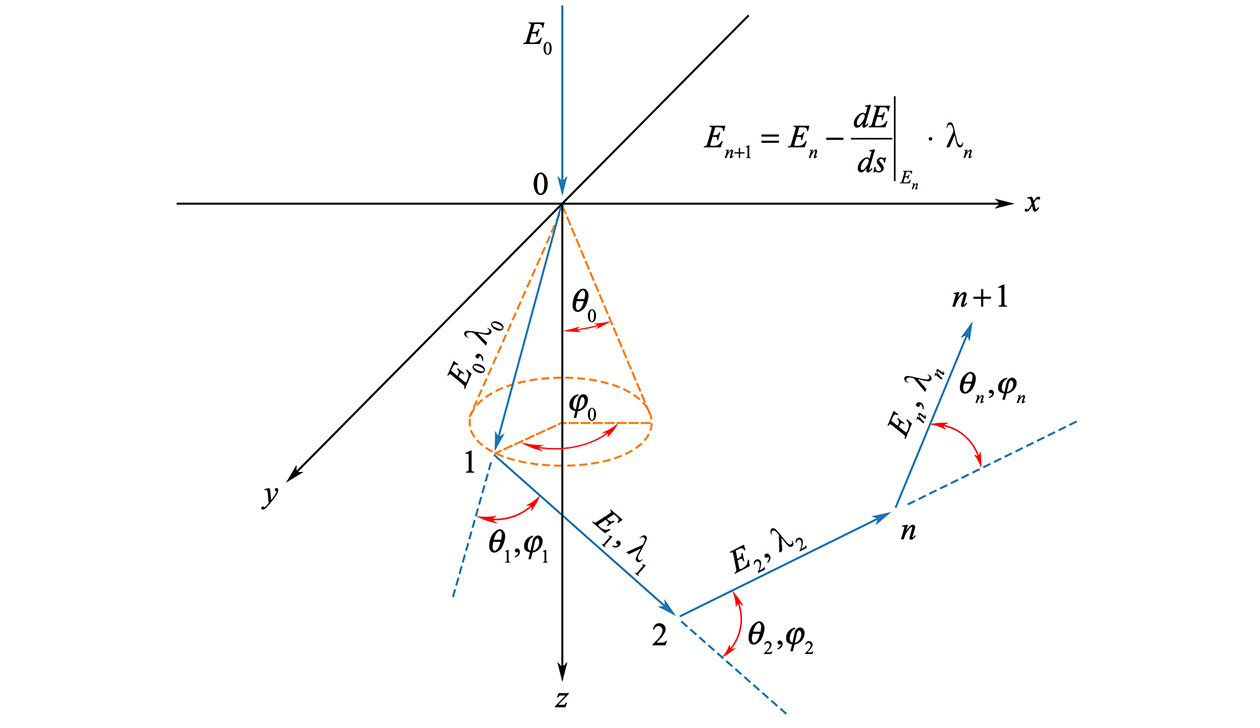
\includegraphics[width=\linewidth]{jpg/MC_200}
	\vspace{-0.5em}
	\caption{Схематическое изображение траектории электрона в веществе, получаемой при моделировании методом Монте-Карло в случае использования модели непрерывных потерь энергии.\vspace{1.5em}}
	\label{fig:Monte_Carlo_scheme}
\end{figure}

\section{Моделирование электронно-стимулированных разрывов полимерных молекул} \label{sec:G_value}
Количественной характеристикой процесса электронно-стимулированной деградации полимерного резиста является радиационно-химический выход разрывов $\Gs$, определяемый как число разрывов полимерных молекул, происходящих при выделении в слое резиста энергии 100 эВ. Экспериментально значение $\Gs$ определяется на основе среднечисловых значений молекулярной массы резиста до и после экспонирования ($\Mn$ и $M_\mathrm{f}$, соответственно), определяемых методом гель-проникающей хроматографии. При известных $\Mn$ и $M_\mathrm{f}$ значение $\Gs$ может быть определено на основе выражения~\cite{Greeneich1979_Mf_Mn}
\begin{equation} \label{eq:G_value_Mn_Mf}
	M_\mathrm{f} = \frac{\displaystyle \Mn}{1 + \frac{\displaystyle \Gs E}{\displaystyle 100 \rho N_\mathrm{A}}},
\end{equation}
где $E$ -- энергия, выделившаяся в слое резиста, $\rho$ -- плотность резиста, $N_\mathrm{A}$ -- число Авогадро.

Исходя из результатов различных экспериментов по измерению $\Gs$, его значение для ПММА при экспонировании электронным лучом при комнатной температуре считается равным 1.8~\cite{Charlesby_1964_Gs}. Также было установлено, что при экспонировании гамма-излучением и электронным лучом при различных температурах ($T$) зависимость $\ln \Gs (1/T)$ близка к линейной (рисунок~\ref{fig:Gs_Charlesby}).

Считается, что электронно-стимулированные разрывы молекул ПММА происходят в результате взаимодействия налетающего электрона с валентными электронами атомов углерода, образующими C---C связь в главной цепи молекулы~\cite{Stepanova_2006}.

\begin{figure}[h]
	\begin{center}
		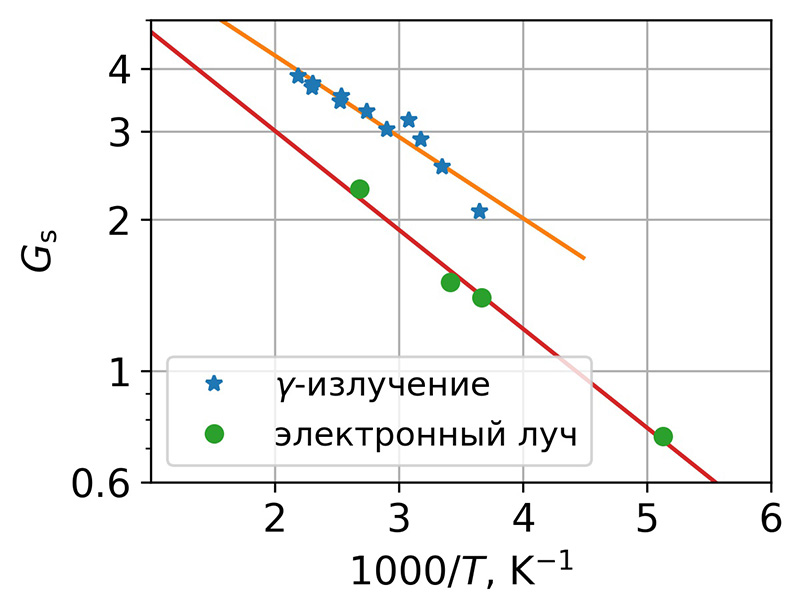
\includegraphics[width=0.55\linewidth]{jpg/Charlesby_G_fit_200}
		\caption{Значения $G_\mathrm{s}$ для ПММА при экспонировании гамма-излучением и электронным лучом, полученные при различных температурах~\cite{Charlesby_1964_Gs}. Сплошная линия отображает аппроксимацию экспериментальных значений $\ln(G_\mathrm{s})$ функцией вида $\alpha\cdot1/T$.}
		\label{fig:Gs_Charlesby}
	\end{center}
\end{figure}

\section{Моделирование термической деполимеризации полимеров} \label{sec:depolymerization}
Термическая деполимеризация полимеров включает в себя процессы возникновения активного центра деполимеризации, его распространения вдоль полимерной молекулы и последующего затухания или переноса на новую молекулу~\cite{Boyd_1}. Кинетические схемы этих процессов могут быть представлены в следующем виде ($P_n$ и $R_n$ -- число стабильных и радикализованных полимерных молекул степени полимеризации $n$ соответственно, $R_\mathrm{E}$ -- концевой радикал):

\begin{center}
	\textbf{Возникновение активного центра деполимеризации}
	\begin{align*}
		P_n \quad \rightarrow \quad & R_r + R_{n-r} \quad & \text{возникновение внутри молекулы} \\
		P_n \quad \rightarrow \quad & R_n + R_\mathrm{E} \quad & \text{возникновение на конце молекулы}
	\end{align*}
	\textbf{Распространение активного центра деполимеризации}
	\begin{align*}
		R_n \quad \rightarrow \quad  R_{n-1} + P_1 \qquad\qquad\qquad\qquad\quad\; \text{$P_1$ -- летучий мономер}
	\end{align*}
	\textbf{Перенос активного центра деполимеризации}
	\begin{align*}
		P_n + R_s \quad \rightarrow \quad & P_r + R_{n-r} + P_s
	\end{align*}
	\textbf{Затухание активного центра деполимеризации}
	\begin{align*}
		R_n \quad \rightarrow \quad & P_n \quad & \text{случайное затухание} \\
		R_r + R_s \quad \rightarrow \quad & P_r + P_s \quad & \text{диспропорционирование} \\
		R_r + R_s \quad \rightarrow \quad & P_{r + s} \quad & \text{рекомбинация}
	\end{align*}
\end{center}
На основе данных кинетические схем можно ввести константы вышеописанных процессов и выразить скорости изменения числа стабильных и радикализованных полимерных молекул за счет каждого из процессов:

%\newpage
\begin{center}
	\textbf{Скорость изменения числа стабильных полимерных молекул} \\
	\textit{уменьшение $P_n$ за счет разрывов внутри молекулы:} \\
	$k_\mathrm{S} (n-1) P_n$ \\
	\textit{уменьшение $P_n$ за счет разрывов на концах молекулы:} \\
	$k_\mathrm{E} P_n$ \\
	\textit{уменьшение $P_n$ за счет переноса активного центра деполимеризации:} \\
	$k_\mathrm{I}(R / V)(n-1) P_n$ \\
	\textit{увеличение $P_n$ за счет переноса активного центра деполимеризации:} \\
	{$\displaystyle k_\mathrm{I} \frac{R_n}{V} \sum_{n=2}^{\infty} n P_n + k_{\mathrm{R}} \frac{R}{V} \sum_{j=n+1}^{\infty} P_j$} \\
	\textit{увеличение $P_n$ за счет уменьшения числа радикалов:} \\
	$k_\mathrm{T} \alpha_n$, $\alpha_n = \left\{
	\begin{array}{l}
		R_n \quad\quad\quad\quad\quad\quad\quad\: \text{реакция 1 порядка} \\
		R_n R / V \quad\quad\quad\quad\quad\: \text{диспропорционирование} \\
		{\displaystyle \frac{1}{2} \sum_{i+j=n}^{\infty} R_i R_j / V} \quad\quad \text{рекомбинация}
	\end{array}\right.$ \\
	($R$ -- полное число радикалов: {$\displaystyle R = \sum_{i=1}^{\infty} R_i$}) \\
	\textbf{Скорость изменения числа радикализованных полимерных молекул} \\
	\textit{увеличение $R_n$ за счет разрывов внутри молекулы:} \\
	$2 k_\mathrm{S} \sum_{j=n+1}^{\infty} P_j$ \\
	\textit{увеличение $R_n$ за счет разрывов на концах молекулы:} \\
	$k_\mathrm{E} P_n$ \\
	\textit{увеличение $R_n$ за счет распространения активного центра деполимеризации:} \\
	$k_\mathrm{P} R_{n+1}$ \\
	\textit{уменьшение $R_n$ за счет распространения активного центра деполимеризации:} \\
	$k_\mathrm{P} R_n$ \\
	\textit{увеличение $R_n$ за счет переноса активного центра деполимеризации:} \\
	${\displaystyle k_\mathrm{I} \frac{R}{V} \sum_{j=n+1}^{\infty} P_j}$ \\
	\textit{уменьшение $R_n$ за счет переноса активного центра деполимеризации:} \\
	${\displaystyle \frac{k_\mathrm{I} R_n}{V} \sum_{n=2}^{\infty} n P_n}$ \\
	\textit{уменьшение $R_n$ за счет уменьшения числа радикалов:} \\
	$k_\mathrm{T} \beta R_n$, $\beta = \left\{
	\begin{array}{l}
		1 \quad\quad\quad \text{реакция 1 порядка} \\
		R / V \quad\;\: \text{диспропорционирование или рекомбинация}
	\end{array}\right.$ \\
\end{center}

Учет всех процессов, приводящих к изменению $P_n$ и $R_n$, позволяет описать состояние полимера системой дифференциальных уравнений:
\begin{equation} \label{eq:kinetic_system_original}
	\left\{
	\begin{aligned}
		&\dots \\
		&\frac{d P_n}{d t} = -(n-1)\left(k_\mathrm{S} + k_\mathrm{I} R / V\right) P_n - k_\mathrm{E} P_n + k_\mathrm{I} R / V \sum_{j=n+1}^{\infty} P_j + k_\mathrm{I} R_n \frac{d_0}{m_0} + k_\mathrm{T} \alpha_n, \\
		&\dots \\
		&\frac{d R_n}{d t} = \left(2 k_\mathrm{S} + k_\mathrm{I} R / V\right) \sum_{j=n+1}^{\infty} P_j + k_\mathrm{E} P_n - \left(\frac{k_\mathrm{I} d_0}{m_0} + k_\mathrm{P} + k_\mathrm{T} \beta\right) R_n + k_\mathrm{P} R_{n+1}, \\
		&\dots \\
		&\frac{d R_1}{d t} = \left(2 k_\mathrm{S} + k_\mathrm{I} R / V\right) \frac{W}{x m_0} + \frac{k_\mathrm{E}}{m_0} \frac{W}{x} - \left(\frac{k_\mathrm{I} d_0}{m_0} + k_\mathrm{T} \beta\right) R_1 + k_\mathrm{P} R_2,
	\end{aligned}
	\right.
\end{equation}
где $m_0$ -- масса мономера, $x$ -- среднечисловая степень полимеризации молекул полимера. 

В исходном виде система \ref{eq:kinetic_system_original} включает в себя 2$N$ уравнений ($N$ -- максимальная степень полимеризации молекул полимера), и ее решение представляет собой трудоемкую задачу -- не в последнюю очередь за счет наличия слагаемых, описывающих эффект переноса активного центра деполимеризации.
Явление переноса активного центра является важной частью процесса полимеризации (в этом случае происходит перенос центра полимеризации)~\cite{chain_transfer_polymerization}, однако его протекание в процессе деполимеризации до сих пор находится под вопросом~\cite{Mita_PMMA_zip_lengths_T}.
Исключение из системы~\ref{eq:kinetic_system_original} слагаемых, отвечающих за перенос активного центра деполимеризации, а также предположение о постоянной концентрации радикализованных молекул существенно упрощают систему~\cite{Boyd_3}:
\begin{equation} \label{eq:Boyd_system_3}
	\left\{
	\begin{aligned}
		&\dots \\
		&d P_n / d t=-(n-1) k_\mathrm{S} P_n + k_\mathrm{R} R_n \bar{R}, \\
		&\dots \\
		&d R_n / d t=2 k_\mathrm{S} \sum_{j=n+1}^{\infty} P_j + k_\mathrm{P}\left(R_{n+1} - R_n\right) - k_\mathrm{T} \bar{R} R_n=0 \quad(n \geq 2), \\
		&\dots \\
		&d R_1 / d t = 2 k_\mathrm{S} \left(W / x m_0\right) + k_\mathrm{P} R_2 - k_\mathrm{T} \bar{R} R_1=0,
	\end{aligned}
	\right.
\end{equation}
где $\bar{R} = R/V$. Здесь и далее учитывается только механизм возникновения центров деполимеризации за счет разрывов в произвольной точке внутри полимерной молекулы (без учета разрывов на концах молекулы).
Дальнейшее суммирование по всем степеням полимеризации приводит систему~\ref{eq:Boyd_system_3} к системе уравнений вида~\cite{Boyd_3}
\begin{equation} \label{eq:moment_equation}
	\frac{d M_i}{d t} = k_\mathrm{S} \left(\frac{2}{i+1} - 1\right) M_{i+1} + \frac{d M_0}{d t} - k_\mathrm{S} M_1 - \frac{i}{\gamma}\left(k_\mathrm{S} M_i + \frac{d M_{i-1}}{dt}\right) \quad(i \geq 1),
\end{equation}
где $1/\gamma = k_\mathrm{P} / (k_\mathrm{T} \bar{R})$ -- средняя длина кинетической цепи при деполимеризации (среднее число свободных мономеров, образующихся вследствие возникновения одного активного центра деполимеризации), $M_i$ -- момент $i$-го порядка молекулярно-массового распределения полимера:
\begin{equation}
	M_i=\sum_{n=2}^{\infty} n^i P_n.
\end{equation}

В качестве функции распределения молекулярной массы полимера может использоваться функция распределения Шульца-Цимма~\cite{Boyd_3, Schulz-Zimm_distribution}, корректно описывающее полимеры, полученные методом радикальной полимеризации~\cite{Schulz-Zimm_distribution_proof}:
\begin{equation} \label{eq:Schulz-Zimm_distribution}
	P_n = C_0 n^z \exp (-n/y).
\end{equation}
Здесь $P_n$ -- число молекул степени полимеризации $n$, $C_0$ -- нормировочный множитель. Параметр $z$ характеризует ширину распределения:
\begin{equation} \label{eq:Schulz-Zimm_1}
	M_\mathrm{w} / M_\mathrm{n} = (z+2) /(z+1),
\end{equation}
где $M_\mathrm{n}$ и $M_\mathrm{w}$ -- среднечисловая и средневесовая молекулярная масса соответственно, а параметр $y$ определяется из выражения
\begin{equation} \label{eq:Schulz-Zimm_2}
	x = y(z+1),
\end{equation}
где $x$ -- среднечисловая степень полимеризации молекул полимера. При этом моменты высших порядков молекулярно-массового распределения полимера могут быть выражены через параметры $y$ и $z$ и момент первого порядка $M_1$:
\begin{equation}
	M_i=M_1 \prod_{n=2}^i(z+n) y^{i-1}.
\end{equation}

Для решения системы~\ref{eq:moment_equation} удобно ввести следующие безразмерные переменные:
\begin{equation} \label{eq:dim_less_MW}
	\begin{aligned}
		\tau & = y_0 k_\mathrm{S} t \\
		\tilde{M}_1 & = M_1 / M_{1_0} \\
		\tilde{y} & = y / y_0 \\
		\tilde{\gamma} & = \gamma y_0 \\
		\tilde{x} & = x / x_0 = \left[y(z+1) / y_0\left(z_0+1\right)\right],
	\end{aligned}
\end{equation}
которые в дальнейшем будут использоваться в уравнениях вида~\ref{eq:moment_equation} для $i$, равного 1, 2 и 3 (величины с нижним индексом ``0'' соответствуют начальному состоянию полимера).
В конечном счете система из этих трех уравнений принимает следующий вид:

\begin{equation} \label{eq:scary_system}
	\begin{aligned}
		&\frac{\tilde{M_1}^{\prime}}{\tilde{M_1}}=\left[\frac{1}{\tilde{y}} \frac{d \tilde{y}}{d \tau}+\frac{1}{(z+1)} \frac{d z}{d \tau}-\tilde{y}(z+1)\right] /[1+\tilde{\gamma} \tilde{y}(z+1)], \\
		&\tilde{y}^{\prime}=(B F-C E) /(A E-D B), \\
		&z^{\prime}=(C D-A F) /(A E-D B),
	\end{aligned}
\end{equation}
где
\begin{equation}
	\begin{aligned}
		&A=-\left[\frac{1}{\tilde{y}[1+\tilde{\gamma} \tilde{y}(z+1)]}+\frac{(z+2) \tilde{\gamma}}{(z+2) \tilde{\gamma} \tilde{y}+2}\right], \\
		&B=-\left[\frac{1}{(z+1)[1+\tilde{\gamma} \tilde{y}(z+1)]}+\frac{\tilde{\gamma} \tilde{y}}{(z+2) \tilde{\gamma} \tilde{y}+2}\right], \\
		&C=\left[\frac{\tilde{y}(z+1)}{\tilde{\gamma} \tilde{y}(z+1)+1}-\frac{\frac{1}{3}(z+2)(z+3) \tilde{\gamma} \tilde{y}^2+2(z+2) \tilde{y}}{(z+2) \tilde{\gamma} \tilde{y}+2}\right], \\
		&D=\left[\frac{(z+2) \tilde{\gamma}}{(z+2) \tilde{\gamma} \tilde{y}+2}-\frac{2(z+2)(z+3) \tilde{\gamma} \tilde{y}+3(z+2)}{(z+2)(z+3) \tilde{\gamma} \tilde{y}^2+3(z+2) \tilde{y}}\right], \\
		&E=\left[\frac{\tilde{\gamma} \tilde{y}}{(z+2) \tilde{\gamma} y+2}-\frac{\tilde{\gamma} \tilde{y}(2 z+5)+3}{(z+2)(z+3) \tilde{\gamma} \tilde{y}+3(z+2)}\right], \\
		&F=\left[\frac{\frac{1}{3}(z+2)(z+3) \tilde{\gamma} \tilde{y}^2+2(z+2) \tilde{y}}{(z+2) \tilde{\gamma} \tilde{y}+2}-\right. \\
		&\left.-\frac{\frac{1}{2}(z+2)(z+3)(z+4)\left(\tilde{\gamma} \tilde{y}^2+3(z+2)(z+3) \tilde{y}\right.}{(z+2)(z+3) \tilde{\gamma} \tilde{y}+3(z+2)}\right].
	\end{aligned}
\end{equation}
Производные в левой части системы~\ref{eq:scary_system} берутся по переменной $\tau$, а сама система решается с использованием численных методов.







\section{Моделирование диффузии мономера в слое полимера}
Ключевая величина, описывающая в процесс диффузии произвольной примеси в слое вещества -- коэффициент диффузии. В настоящее время существуют два основных подхода к определению коэффициента диффузии мономера (метилметакрилат, ММА) в слое ПММА. Первый из них основан на использовании теории свободного объема, которая позволяет непосредственно определить коэффициент диффузии на основе различных параметров вещества. Второй подход основан на косвенном определении коэффициента диффузии за счет моделирования выхода мономера из слоя ПММА и сравнения результатов моделирования с экспериментальными данными.

\subsection{Теория свободного объема}
Точный расчет коэффициента диффузии частиц примеси в слое полимера возможен на основе теории свободного объема~\cite{Vrentas_free_volume, Zielinski_free_volume}:
\begin{equation}
	\ln D=\ln \bar{D}_0-\frac{E^*}{\mathrm{R} T}-\left\{\frac{\left(1-\omega_2\right) \hat{V}_1^*+\xi \omega_2 \hat{V}_2^*}{\hat{V}_{\mathrm{FH}} / \gamma}\right\}.
\end{equation}
Здесь $E^*$ -- энергия, необходимая для преодоления сил притяжения в пересчете на 1 моль примеси, $R$ -- универсальная газовая постоянная, $T$ -- температура, $\bar{D}_0$, $\xi$ и $\gamma$ -- параметры, $\hat{V}_1^*$ и $\hat{V}_2^*$ -- удельные объемы полимера и примеси, соответственно, $\hat{V}_{\mathrm{FH}}$ -- средний свободный объем полостей в смеси полимера и примеси, $\omega_2$ -- массовая доля полимера в смеси. Величина $\hat{V}_{\mathrm{FH}} / \gamma$ определяется выражением
\begin{equation}
	\hat{V}_{\mathrm{FH}} / \gamma=\left(1-\omega_2\right)\left(\frac{K_{11}}{\gamma_1}\right)\left(K_{21}+T-T_{\mathrm{g} 1}\right)+\omega_2 \hat{V}_{\mathrm{FH} 2} / \gamma_2,
\end{equation}
где $\left(K_{11} / \gamma_1\right)$ и $\left(K_{21}-T_\mathrm{g1} 1\right)$ -- параметры примеси, величина $\hat{V}_{\mathrm{FH} 2} / \gamma_2$ описывает вклад полимерной матрицы в средний свободный объем полостей. Эта величина зависит от того, выше или ниже температуры стеклования полимера ($T_\mathrm{g2}$) находится температура системы:
\begin{equation}
	\begin{aligned}
		&\hat{V}_\mathrm{FH2} =
		\hat{V}_2^0 (T_{g2}) \left[ f_{H2}^{G}+\alpha_2 (T-T_{g2}) \right], & T \geq T_\mathrm{g2} \\
		&\hat{V}_\mathrm{FH2} =
		\hat{V}_2^0 (T_{g2})\left[f_\mathrm{H2}^{G}+(\alpha_2-\alpha_{c2})(T-T_{g2})\right], \hspace{1em} & T<T_\mathrm{g2}
	\end{aligned}
\end{equation}
В этом выражении $\hat{V}_2^0\left(T_{\mathrm{g} 2}\right)$ -- удельный объем полимера при температуре $T_\mathrm{g2}$, \linebreak $\alpha_2$ -- коэффициент температурного расширения полимера в состоянии равновесия, $f_{\mathrm{H} 2}^{\mathrm{G}}$ -- доля объема пустот в полимере при температуре $T_\mathrm{g2}$:
\begin{equation}
	f_{\mathrm{H} 2}^{\mathrm{G}}=\alpha_2 K_{22},
\end{equation}
\begin{equation}
	\alpha_{\mathrm{c} 2}=\frac{1}{T_{\mathrm{g} 2}} \ln \left(\frac{\hat{V}_2^0\left(T_{\mathrm{g} 2}\right)\left(1-f_{\mathrm{H} 2}^{\mathrm{G}}\right)}{\hat{V}_2^0(0)}\right),
\end{equation}
\begin{equation}
	\gamma_2=\frac{\hat{V}_2^0\left(T_{\mathrm{g} 2}\right) \alpha_2}{\left(K_{12} / \gamma_2\right)},
\end{equation}
\begin{equation}
	\hat{V}_1^*=\hat{V}_1^0(0); \hspace{1em} \hat{V}_2^*=\hat{V}_2^0(0),
\end{equation}
где $K_{22}$ и $\left(K_{12} / \gamma_2\right)$ -- параметры модели свободного объема, $\hat{V}_1^0(0)$ и $\hat{V}_2^0(0)$ -- удельные объемы примеси и полимера в состоянии равновесия при $T=0$ K. Параметры модели свободного объема для диффузии ММА в слое ПММА приведены в таблице~\ref{table:D_free_volume}~\cite{Tonge_free_volume_parameters}.

\begin{table}[h]
	\centering
	\caption{Параметры модели свободного объема для диффузии ММА в ПММА.}
	\begin{tabular}{l c l}
		\hline \hline \\ [-1em]
		Параметр & \hspace{4em} & Значение
		\\ \hline \\ [-1em]
		$\hat{V}_1^0(0)$, см$^\text{-1}$ & \hspace{1em} & 0.871
		\\ \\ [-1em]
		$\tilde{V}_1^0(0)$, см$\ppp$ моль$^\text{-1}$ & \hspace{1em} & 86.9
		\\ \\ [-1em]
		$\hat{V}_2^0(0)$, см$\ppp$ г$^\text{-1}$ & \hspace{1em} & 0.762
		\\ \\ [-1em]
		$\tilde{V}_2^*$, см$\ppp$ моль$^\text{-1}$ & \hspace{1em} & 135
		\\ \\ [-1em]
		$f_\mathrm{H2}^\mathrm{G}$ & \hspace{1em} & 0.00456
		\\ \\ [-1em]
		$K_{22}$, К & \hspace{1em} & 80
		\\ \\ [-1em]
		$(K_{12} / \gamma_2)$, см$\ppp$ г$^{-1}$ К$^\text{-1}$ & \hspace{1em} & 1.28\:$\cdot$\,10$^\text{-4}$
		\\ \\ [-1em]
		$\gamma_2$ & \hspace{1em} & 3.88
		\\ \\ [-1em]
		$\alpha_\mathrm{c2}$, К$^\text{-1}$ & \hspace{1em} & 2.37\:$\cdot$\,10$^\text{-4}$
		\\ \\ [-1em]
		$\xi_\mathrm{L}$ & \hspace{1em} & 0.64
		\\ \\ [-1em]
		$\xi$ & \hspace{1em} & 0.58
		\\ \\ [-1em]
		$E^*$, Дж моль$^\text{-1}$ & \hspace{1em} & 0.58
		\\ \\ [-1em]
		$\bar{D}_0$, см$\pp$ с$^\text{-1}$ & \hspace{1em} & 1.27\:$\cdot$\,10$^\text{-3}$
		\\ \\ [-1em]
		$(K_{11} / \gamma_1)$, см$\ppp$ г$^\text{-1}$ К$^\text{-1}$ & \hspace{1em} & 6.91\:$\cdot$\,10$^\text{-4}$
		\\ \\ [-1em]
		$(K_{21}-T_\mathrm{g1})$, К & \hspace{1em} & 72.26
		\\ \\ [-1em]
		$\hat{V}_2^0(T_\mathrm{g2})$, см$\ppp$ г$^\text{-1}$ & \hspace{1em} & 0.8754
		\\ \\ [-1em]
		$\tilde{V}_\mathrm{c}$, см$\ppp$ моль$^\text{-1}$ & \hspace{1em} & 311 \\ \hline \hline
	\end{tabular}
	\label{table:D_free_volume}
\end{table}

Вычисление параметров теории свободного объема зачастую является затруднительным, и для определения коэффициента диффузии примеси в полимере может быть использован подход, основанный на масштабировании известных коэффициентов диффузии. Таким образом, в работе~\cite{Karlsson2001_diffusion} было выведено универсальное выражение для коэффициента диффузии малой примеси в полимере:
\begin{equation} \label{eq:Karlsson_diffusion}
	\log D (w_\mathrm{p}, \Delta T) = C_1 - w_p C_2 + \Delta T C_3 + w_p \Delta T C_4,
\end{equation}
значения параметров $C_1$, $C_2$, $C_3$ и $C_4$ которого для различных значений массовой доли полимера $w_\mathrm{p}$ приведены в таблице~\ref{table:Karlsson_diffusion}.

\begin{table}[h]
	\begin{center}
		\caption{Значения параметров $C_1$, $C_2$, $C_3$ и $C_4$ функции~\ref{eq:Karlsson_diffusion} для различных областей значений $w_\mathrm{p}$.}
		\begin{tabular}{lc rc rc rc r}
			\hline \hline \\ [-1em]
			Область $w_\mathrm{p}$ & \hspace{1em} & $C_1$ & \hspace{1em} & $C_2$ & \hspace{1em} & $C_3$ & \hspace{1em} & $C_4$
			\\ \hline \\ [-1em]
			$0 \leq w_\mathrm{p} \leq 0.795$ & \hspace{1em} & 24.428 & \hspace{1em} & 1.842 & \hspace{1em} & 0 & \hspace{1em} & 8.12\:$\cdot$\,10$^\text{-3}$
			\\ \\ [-1em]
			$0.795 \leq w_\mathrm{p} \leq 0.927$ & \hspace{1em} & 26.0 & \hspace{1em} & 37.0 & \hspace{1em} & 0.0797 & \hspace{1em} & 0
			\\ \\ [-1em]
			$0.927 \leq w_\mathrm{p} \leq 0.945$ & \hspace{1em} & 159.0 & \hspace{1em} & 170.0 & \hspace{1em} & 0.3664 & \hspace{1em} & 0
			\\ \\ [-1em]
			$0.945 \leq w_\mathrm{p} \leq 1$ & \hspace{1em} & 213.7 & \hspace{1em} & 0.5 & \hspace{1em} & 0 & \hspace{1em} & 0
			\\ \hline \hline
		\end{tabular}
		\label{table:Karlsson_diffusion}
	\end{center}
\end{table}


\subsection{Модель выхода мономера из слоя полимера}
В работе~\cite{Fragala_3_diffusion} проводилось исследование выхода мономера из слоя \linebreak ПММА при его экспонировании ионным лучом. В модели процесса ионно-стимулированной деполимеризации ПММА учитывались процессы инициирования и роста кинетической цепи:

\begin{equation}
	\begin{aligned}
		&{[\text { Полимер }]_N \stackrel{\text { Экспонирование }}{\longrightarrow}[\text { Полимер }]_{N-m}+[\text { Радикал }]_m,} \\
		&{[\text { Радикал }]_m \stackrel{\text { Деполимеризация }}{\longrightarrow} \text { Мономер }+[\text { Радикал }]_{m-1} .}
	\end{aligned}
\end{equation}
Концентрация активных центров деполимеризации ($c_\mathrm{I}$) описывалась уравнением
\begin{equation}
	\frac{\partial c_\mathrm{I}}{\partial t} = K_\mathrm{I} f(t) - K_\mathrm{P} c_\mathrm{I},
\end{equation}
где $K_\mathrm{I}$ и $K_\mathrm{P}$ -- константы скоростей инициирования и роста кинетической цепи соответственно, а функция $f(t)$ описывает режим работы ионного луча:
\begin{equation}
	f(t) = 1 - H(t - t_0),
\end{equation}
где $H(t)$ -- функция Хевисайда,  $t_0$ -- время работы ионного луча.

Образование мономера предполагалось однородным по объему полимера, что позволило описать процесс выхода мономера одномерным уравнением диффузии:
\begin{equation} \label{eq:raduino_diff_eq}
	\frac{\partial c_\mathrm{M}}{\partial t} = D\left(\frac{\partial^2 c_\mathrm{M}}{\partial z^2}\right) + \beta K_\mathrm{P} c_\mathrm{I},
\end{equation}
где $c_\mathrm{M}$ -- концентрация мономера, $D$ -- коэффициент диффузии мономера в слое ПММА, считающийся постоянным по всему объему слоя, $\beta$ -- среднее число свободных мономеров, образующихся в результате появления одного активного центра деполимеризации. Уравнение~\ref{eq:raduino_diff_eq} дополнялось начальными и граничными условиями, описывающими беспрепятственный переход мономера через границу ПММА/вакуум, отражение мономера от подложки и его отсутствие до и по истечении большого времени после экспонирования:
\begin{equation} \label{eq:diff_eq_conditions}
	\begin{aligned}
		&\left.c_\mathrm{M}\right|_{z=z_0} = 0, \\
		&\left.\frac{\partial c_\mathrm{M}}{\partial z}\right|_{z=0} = 0, \\
		&\left.c_\mathrm{M}\right|_{t=0} = 0, \\
		&\lim _{t \rightarrow \infty} c_\mathrm{M} = 0, \\
		&\lim _{t \rightarrow \infty} c_\mathrm{I} = 0,
	\end{aligned}
\end{equation}
где $z=0$ и $z=z_0$ -- границы слоя ПММА.

Решение уравнения~\ref{eq:raduino_diff_eq} с условиями~\ref{eq:diff_eq_conditions} позволило рассчитать поток мономера через границу полимер/вакуум во время экспонирования ($t < t_0$):
\begin{equation}
	\begin{aligned}
		J_{+}(t)= & A \beta K_\mathrm{I} z_0
		\left[
		1 - \frac{8}{\pi^2} \sum_{n=1}^{\infty}
		\frac{1}{(2n-1)^2} \frac{1}{(1 - \alpha_n / K_\mathrm{P})} \times \right. \\ & \left.
		\times
		\left(
			\exp (-\alpha_n t)-\frac{\alpha_n}{K_\mathrm{P}} \exp (-K_\mathrm{P} t)
		\right)
		\right]
	\end{aligned}
\end{equation}
и после экспонирования ($t > t_0$):
\begin{equation}
	\begin{aligned}
		J_{-}(t)= A \beta K_i z_0 \left[
			\frac{8}{\pi^2} \sum_{n=1}^{\infty} \frac{1}{(2 n-1)^2} \frac{1}{\left(1-\alpha_n / K_\mathrm{P}\right)}\right. \times \quad \quad \quad \quad \\
	\times \left.
	\left(
	\exp (-\alpha_n t) (\exp (\alpha_n t_0)-1)- \frac{\alpha_n}{K_\mathrm{P}}
	\exp (-K_\mathrm{P} t) (\exp (K_\mathrm{P} t_0)-1)
	\right)
	\right].
	\end{aligned}
\end{equation}

Параметры модели $K_\mathrm{I}$, $K_\mathrm{P}$ и $\beta$ были подобраны за счет сравнения промоделированной зависимости потока мономера от времени с экспериментальной, что позволило определить коэффициент диффузии ММА в ПММА при температурах эксперимента~(таблица~\ref{table:Ki_Kp_D}).

\begin{table}[h]
	\begin{center}
	\caption{Константы скоростей инициирования и роста кинетической цепи при ионно-стимулированной термической деполимеризации ПММА и коэффициенты диффузии ММА в ПММА, полученные в работе~\cite{Fragala_3_diffusion} для различных температур.}
	\begin{tabular}{lc rc rc r}
		\hline \hline \\ [-1em]
		Температура, $^\circ$C & \hspace{4em} & $K_\mathrm{I} \beta$, с$^\text{-1}$ & \hspace{1em} & $K_\mathrm{P}$, с$^\text{-1}$ & \hspace{1em} & $D$, см$\pp$с$^\text{-1}$
		\\ \hline \\ [-1em]
		135 & \hspace{4em} & 7\:$\cdot$\,10$^\text{-4}$ & \hspace{1em} & 90 & \hspace{1em} & 2\:$\cdot$\,10$^\text{-10}$
		\\ \\ [-1em]
		150 & \hspace{4em} & 1.85\:$\cdot$\,10$^\text{-3}$ & \hspace{1em} & 100 & \hspace{1em} & 3.5\:$\cdot$\,10$^\text{-10}$
		\\ \\ [-1em]
		160 & \hspace{4em} & 1.6\:$\cdot$\,10$^\text{-3}$ & \hspace{1em} & 100 & \hspace{1em} & 1.1\:$\cdot$\,10$^\text{-9}$
		\\ \\ [-1em]
		170 & \hspace{4em} & 3.2\:$\cdot$\,10$^\text{-3}$ & \hspace{1em} & 120 & \hspace{1em} & 1.2\:$\cdot$\,10$^\text{-9}$
		\\ \\ [-1em]
		185 & \hspace{4em} & 3.1\:$\cdot$\,10$^\text{-3}$ & \hspace{1em} & 300 & \hspace{1em} & 2.1\:$\cdot$\,10$^\text{-9}$
		\\ \hline \hline
	\end{tabular}
	\label{table:Ki_Kp_D}
	\end{center}
\end{table}

Среднечисловая молекулярная масса ПММА, использовавшегося в проводимых экспериментах составляла около 30000, и для образцов ПММА с другой среднечисловой молекулярной массой коэффициенты диффузии могут отличаться. Для учета зависимости коэффициента диффузии мономера в полимере от молекулярной массы полимера может быть использовано эмпирическое соотношение, полученное в работе~\cite{Berens_diffusion_Mn} для полистирола:
\begin{equation} \label{eq:diffusion_Mn}
	\lg D = \lg D_\infty + k / M_\mathrm{n},
\end{equation}
где $D_\infty$ -- коэффициент диффузии, соответствующий условно бесконечной среднечисловой молекулярной массе полимера ($\Mn$), значение параметра $k$ составляет (1.06~$\pm$~0.46)\:$\cdot$\,10$^\text{4}$.

\section{Моделирование термического растекания резиста}


\subsection{Аналитический подход}
Моделирование растекания резиста может быть проведено аналитически на основе подхода, предложенного для моделирования термического растекания периодических структур, полученных в резисте методом НИЛ~\cite{Leveder_2008, Leveder_2011}. В основе этого подхода лежит Фурье-преобразование профиля резиста $h(t)$:
\begin{equation}
	\begin{aligned}
		& h(x, t) = h_0 + \tilde{h}(x, t), \\
		& \tilde{h}(x, t) = \sum_{-\infty}^{+\infty} a_n(t) \exp \left(i n \frac{2 \pi}{\lambda} x\right),
	\end{aligned}
\end{equation}
где $h_0$ -- средняя высота профиля, $\lambda$ -- пространственный период профиля.

Уравнение Навье-Стокса при условии отсутствия проскальзывания и с учетом расклинивающего и Лапласова давления может быть представлено в следующем виде:
\begin{equation} \label{eq:Navier-Stokes}
	\partial_t \tilde{h}-\frac{A}{6 \pi \eta h_0} \partial_x^2 \tilde{h}+\frac{\gamma h_0^3}{3 \eta} \partial_x^4 \tilde{h} = 0,
\end{equation}
где $A$ -- постоянная Гамакера, $\gamma$ -- коэффициент поверхностного натяжения резиста, $\eta$ -- вязкость резиста. Решение уравнения~\ref{eq:Navier-Stokes} приводит к выражению для времени затухания $n$-й пространственной гармоники профиля ($\tau_n$):
\begin{equation}
	\frac{1}{\tau_n}=\left(n \frac{2 \pi}{\lambda}\right)^2 \frac{A}{6 \pi h_0 \eta}+\left(n \frac{2 \pi}{\lambda}\right)^4 \frac{\gamma h_0^3}{3 \eta}.
\end{equation}
При выполнении условия $\left(\frac{\displaystyle h_0^2}{\displaystyle \lambda}\right)^2 \ll \frac{\displaystyle A}{\displaystyle \gamma}$ выражение для $\tau_n$ принимает более простой вид:
\begin{equation}
	\tau_n=\frac{3 \eta}{\gamma h_0^3} \times\left(\frac{\lambda}{2 \pi n}\right)^4.
\end{equation}
Результирующий профиль в момент времени $t$ определяется суммой гармоник (рисунок~\ref{fig:ferlow_analytical}):
\begin{equation}
	\tilde{h}(x, t)=\sum_{-\infty}^{+\infty} a_n(0) \exp \left(-\frac{t}{\tau_n}+i n \frac{2 \pi}{\lambda} x\right).
\end{equation}

\begin{figure}
	\begin{center}
		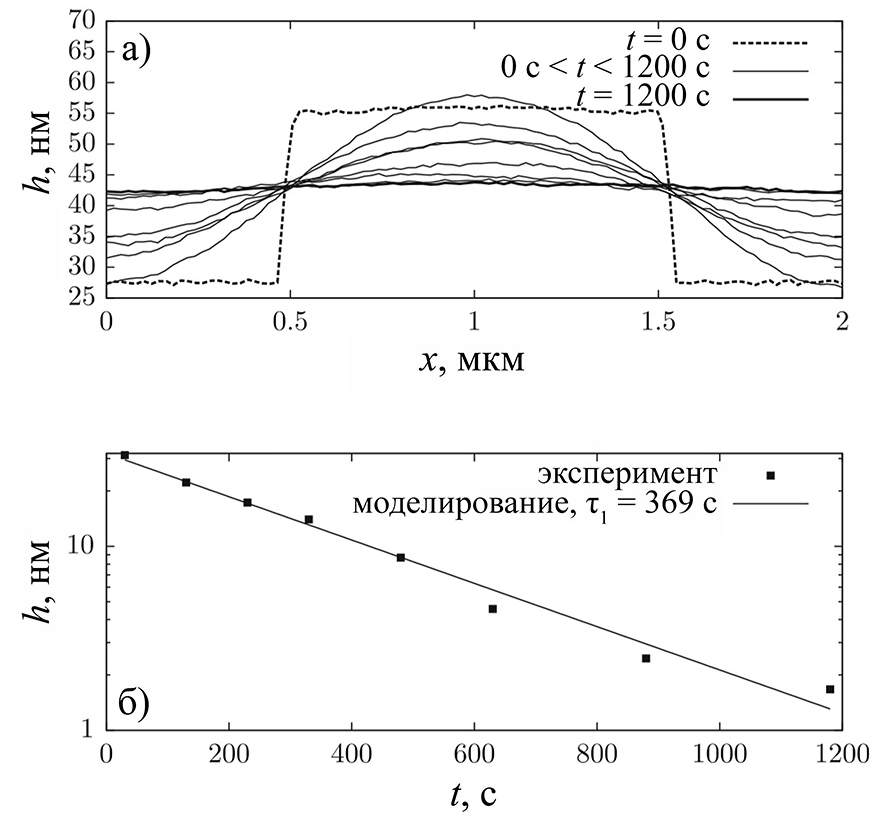
\includegraphics[width=0.7\linewidth]{jpg/reflow_Leveder_large_200}
		\caption{Растекание решетки с периодом 2 мкм, полученной в ПММА методом наноимпринтной литографии~\cite{Leveder_2011}. Нагрев производился при температуре 145~$^\circ$С, время нагрева составляло от 50 до 1200 с: а) 2D профили, полученные методом атомно-силовой микроскопии, б) зависимость высоты профиля решетки от времени в эксперименте (точки) и при моделировании со значением $\tau_1$ = 369 c (сплошная линия).}
		\label{fig:ferlow_analytical}
	\end{center}
\end{figure}

Следует отметить, что вязкость резиста зависит как от температуры резиста, так и от его молекулярной массы. Температурная зависимость вязкости резиста может быть описана уравнением Вильямса-Ландела-Ферри~\cite{bird1987dynamics_WLF}:
\begin{equation} \label{eq:WLF}
	\log \left( \frac{\eta(T)}{\eta(T_0)} \right) = -\frac{C_1(T-T_0)}{C_2+(T-T_0)},
\end{equation}
где $T$ -- температура резиста, значения $\eta(T_0)$, $C_1$, $C_2$ и $T_0$ для различных резистов приведены в таблице~\ref{table:WLF}~\cite{aho2008measurement_WLF}.

Зависимость вязкости резиста от его молекулярной массы может быть описана эмпирической формулой:
\begin{equation} \label{eq:3p4_3p1}
	\eta \propto \Mn^\alpha,
\end{equation}
где $\Mn$ -- среднечисловая молекулярная масса резиста, значение параметра $\alpha$ для ПММА составляет 3.4 при $\Mn$ $\geq$ 48000 и 1.4 при $\Mn$ $<$ 48000~\cite{Leveder_2010, Bueche_3p4_1p4}.

\begin{table}[h]
	\centering
	\caption{Значения параметров функции~\ref{eq:WLF} для полистирола (ПС), полиметилметакрилата (ПММА) и поликарбоната (ПК)~\cite{aho2008measurement_WLF}.}
	\begin{tabular}{l c c c}
		\hline \hline \\ [-1em]
		Параметр \hspace{2em} & ПС \hspace{2em} & ПММА \hspace{2em} & ПК
		\\ \hline \\ [-1em]
		$\eta(T_0)$, Па с \hspace{2em} & 7310.4 \hspace{2em} & 13450 \hspace{2em} & 2763
		\\ \\ [-1em]
		$C_1$ \hspace{2em} & 10.768 \hspace{2em} & 7.6682 \hspace{2em} & 4.7501
		\\ \\ [-1em]
		$C_2$, $^\circ$C \hspace{2em} & 289.21 \hspace{2em} & 210.76 \hspace{2em} & 110.12
		\\ \\ [-1em]
		$T_0$, $^\circ$C \hspace{2em} & 190 \hspace{2em} & 200 \hspace{2em} & 200
		\\ \hline \hline
	\end{tabular}
\label{table:WLF}
\end{table}


\subsection{Численный подход}
Второй подход к моделированию растекания профиля резиста основан на использовании численного метода конечных элементов, реализованном в программе ``Surface Evolver''~\cite{Brakke_SE}. В этом подходе структурные свойства трехмерного объекта задаются свойствами его поверхности, и эволюция формы объекта в различных процессах описываются изменением формы его поверхности. Моделирование эволюции формы объекта проводится путем минимизации полной поверхностной энергии, при этом объем внутри поверхности на протяжении процесса моделирования поддерживается постоянным. В процессе моделирования поверхность объекта разбивается на треугольные площадки -- грани, задаваемыми тремя узлами -- вершинами, которые, в свою очередь, соединяются ориентированными ребрами (рисунок~\ref{fig:SE_12}). Энергия отдельной грани вычисляется по формуле
\begin{equation}
	E_i=\frac{\gamma_i}{2}\left\|\vec{e}_0 \times \vec{e}_1\right\|,
\end{equation}
где $\gamma_i$ -- коэффициент поверхностного натяжения грани с номером $i$. Сила, действующая на вершину $V_0$ (рисунок~\ref{fig:SE_12}), определяется выражением
\begin{equation}
	\vec{F}_{V_0}=\frac{\gamma_i}{2} \cdot \frac{\vec{e}_1 \times\left(\vec{e}_0 \times \vec{e}_1\right)}{\left\|\vec{e}_0 \times \vec{e}_1\right\|}.
\end{equation}

При моделировании растекания двумерных структур в резисте последние представляются в виде фигуры бесконечной протяженности. При этом моделирование проводится для участка фигуры конечной длины с использованием зеркальных граничных условия на краях участка (рисунок~\ref{fig:SE_3}). Таким образом, возникают три возможных типа граней -- грани на границе полимер/вакуум (p), грани на границе полимер/подложка (ps) и боковые (зеркальные) грани (m). Полная энергия поверхности $E_\mathrm{tot}$ вычисляется по формуле
\begin{equation}
	E_\mathrm{tot} = E_\mathrm{p} - (E_\mathrm{ps} + E_\mathrm{m}),
\end{equation}
где 
\begin{equation}
	E_\mathrm{x} = \sum_{i} E_{\mathrm{x},i}, \hspace{0.5em} \mathrm{x} = \mathrm{p}, \mathrm{ps}, \mathrm{m}.
\end{equation}

\begin{figure}
	\begin{minipage}{0.55\textwidth}
		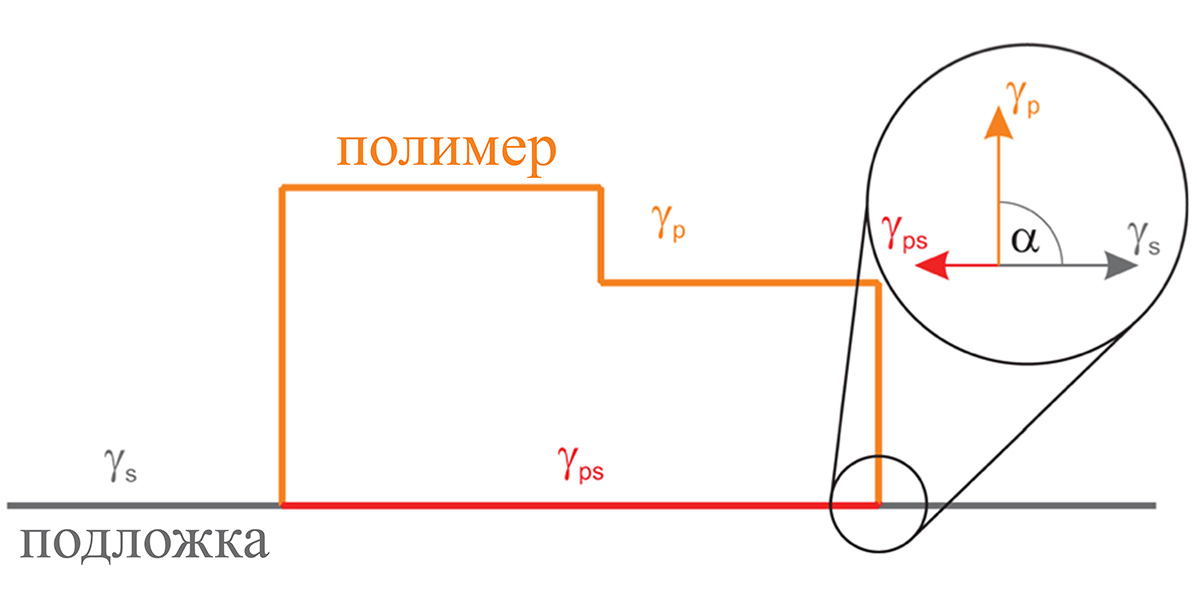
\includegraphics[width=\linewidth]{jpg/SE_1_200}
	\end{minipage}
	\begin{minipage}{0.4\textwidth}
		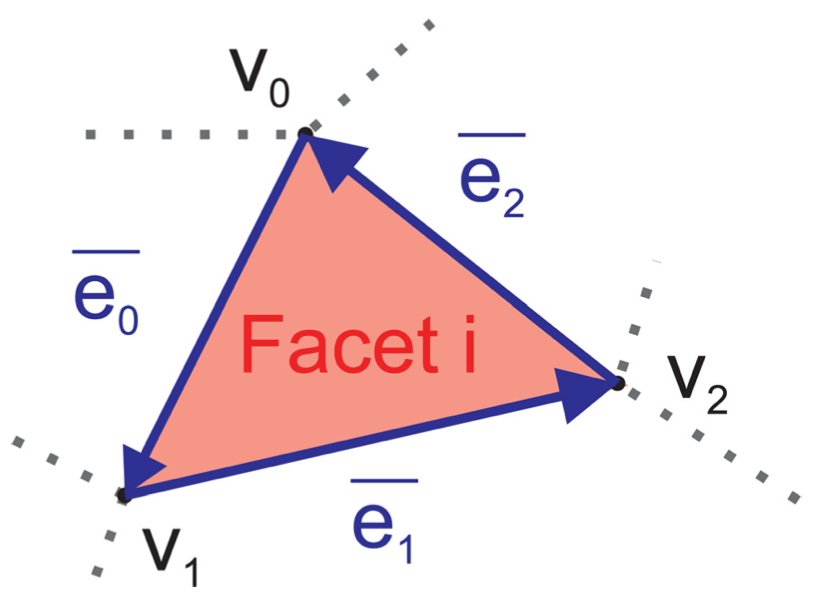
\includegraphics[width=\linewidth]{jpg/SE_2}
	\end{minipage}
	\vspace{0.5em}
	\caption{Схематическое изображение поверхности, заданной в программе ``Surface~Evolver''. $\gamma_\mathrm{p}$, $\gamma_\mathrm{s}$ и $\gamma_\mathrm{ps}$ -- коэффициенты поверхностного натяжения для поверхности полимера, подложки и границы полимер-подложка соответственно, $v_1$, $v_2$ и $v_3$ -- вершины, образующие $i$-ю грань поверхности, $\vec{e_1}$, $\vec{e_2}$ и $\vec{e_3}$ -- ориентированные ребра грани.}
	\label{fig:SE_12}
\end{figure}

В работах по использованию программы ``Surface~Evolver'' для моделирования растекания слоя ПММА моделирование проводилось в режиме нормализации площади, использующемся для реалистичного описания движения под действием сил поверхностного натяжения~\cite{Kirchner_reflow}. В этом режиме при вычислении силы, действующей на вершину, учитывается площадь всех граней, окружающих вершину. Поскольку каждая грань задается тремя вершинами,
сила, действующая на каждую из вершин, будет обратно пропорциональна 1/3 от суммарной площади всех граней, окружающих данную вершину ($A$):
\begin{equation}
	\vec{F}_\mathrm{norm} = \frac{\vec{F}}{A/3} = \frac{3\vec{F}}{A}.
\end{equation}

Связь силы, действующей на вершину, со скоростью движения вершины в процессе моделирования эволюции поверхности описывается коэффициентом подвижности вершины $\mu$:
\begin{equation} \label{eq:SE_v}
	\vec{v} = \vec{F}_\mathrm{norm} \cdot \mu = \frac{\vec{F}}{A/3} \cdot \mu.
\end{equation}
Смещение вершины определяется формулой
\begin{equation} \label{eq:SE_delta}
	\boldsymbol{\delta} = \vec{v} \cdot s,
\end{equation}
где $s$ -- величина, называющаяся ``scale'' и использующаяся в качестве временной переменной.

Следует отметить, что в исходном виде данный метод применяется только для определения конечной формы поверхности, поскольку связь величины $s$ со временем, а также связь подвижности вершин поверхности с физическими величинами, описывающими слой полимера, до настоящего времени не были известны.


\begin{figure}[t]
	\begin{center}
		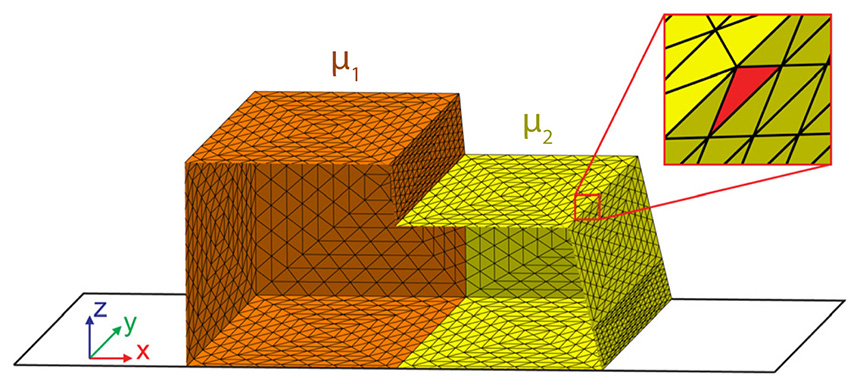
\includegraphics[width=0.9\linewidth]{jpg/SE_3_medium}
		\vspace{1em}
		\caption{Модель поверхности образца, полученного методом полутоновой литографии, заданная в программе ``Surface Evolver''~\cite{Kirchner_reflow}. Поверхность состоит из двух частей с различными значениями подвижности вершин ($\mu_1$ и $\mu_2$).}
		\label{fig:SE_3}
	\end{center}
\end{figure}

\section{Моделирование нагрева резиста при экспонировании} \label{sec:sim_heating}

Выделение энергии в резисте при экспонировании может приводить к повышению его температуры, что может повлиять на масштаб процессов деполимеризации, диффузии и растекания. В работах по моделированию нагрева резиста при экспонировании часто рассматривается случай плоского слоя резиста, расположенного на поверхности полубесконечной подложки~\cite{Cui_heating} (рисунок~\ref{fig:heating_paper}). В этом случае уравнение теплопроводности принимает следующий вид:
\begin{equation} \label{eq:heat_diffusion}
	\begin{aligned}
		& \frac{\partial T_1}{\partial t}-k_1\left(\frac{\partial^2 T_1}{\partial x^2}+\frac{\partial^2 T_1}{\partial y^2}+\frac{\partial^2 T_1}{\partial z^2}\right) = h(x, y, z, t), \quad 0 < z \leqslant d, \\
		& \frac{\partial T_2}{\partial t}-k_2\left(\frac{\partial^2 T_2}{\partial x^2}+\frac{\partial^2 T_2}{\partial y^2}+\frac{\partial^2 T_2}{\partial z^2}\right) = h(x, y, z, t), \quad d \leqslant z < \infty.
	\end{aligned}
\end{equation}
Здесь $d$ -- толщина слоя резиста, $k_i = D_i / \rho_i c_{\mathrm{v} i}$ ($i=1,2$), $h=S / \rho c_\mathrm{v}$, $D_i$, $\rho_i$ и $c_{\mathrm{v} i}$  -- коэффициент теплопроводности, плотность и удельная теплоемкость резиста ($i=1$) или подложки ($i=2$). Величина $S$, определяющая скорость выделения тепла в резисте при экспонировании, может быть рассчитана по формуле
\begin{equation}
	S(x, y, z, t)=\frac{E_0 Q \lambda(\xi)}{R_{\mathrm{g}} t_{\mathrm{e}}},
\end{equation}
где $E_0$ -- энергия электронного пучка, $Q$, $t_\mathrm{e}$ -- доза и время экспонирования, соответственно, $R_\mathrm{g}$ -- радиус Грюна:
\begin{equation}
	R_{\mathrm{g}}=\frac{4.6 \times 10^{-2}}{\rho} E_0^{1.75},
\end{equation}
а для определения энергии, выделившейся в резисте на глубине $z$ используется эмпирическая функция $\lambda(\xi)$ с параметрами $b_i$~\cite{Everhart_lambda}:
\begin{equation}
	\begin{aligned}
	& \lambda(\xi) = b_0+b_1 \xi+b_2 \xi^2+b_3 \xi^3, \\
	& \xi=z/R_\mathrm{g}.
	\end{aligned}
\end{equation}

\begin{figure}
	\centering
	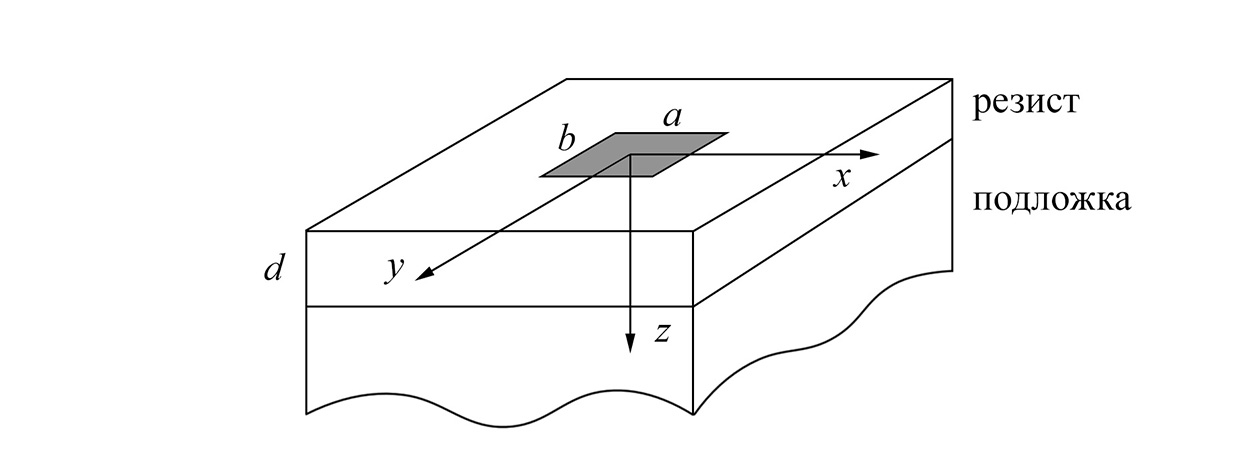
\includegraphics[width=0.9\linewidth]{jpg/heating_paper_200}
	\caption{Система координат и обозначения, используемые при моделировании нагрева резиста в процессе экспонировании~\cite{Cui_heating}.}
	\label{fig:heating_paper}
\end{figure}
Граничные условия для уравнения~\ref{eq:heat_diffusion} имеют вид:
\begin{equation} \label{eq:heat_diff_eq_conditions}
	\begin{aligned}
		\left.\frac{\partial T_1}{\partial z}\right|_{z=0} &= 0, \\
		D_1 \left.\frac{\partial T_1}{\partial z}\right|_{z=d} &= D_2 \left.\frac{\partial T_2}{\partial z}\right|_{z=d}, \\
		\left.T_1\right|_{z=d} &= \left.T_2\right|_{z=d}, \\
		\lim _{z \rightarrow \infty} T_2 &= 0, \\
		\lim _{(x,y) \rightarrow (\infty, \infty)} T_1 &= \lim _{(x,y), \rightarrow (\infty, \infty)} T_2 = 0.
	\end{aligned}
\end{equation}
Решение уравнения~\ref{eq:heat_diffusion} с граничными условиями~\ref{eq:heat_diff_eq_conditions} выражается в следующем виде:
\begin{equation} \label{eq:heat_final_equation}
	\begin{split}
		T(x, y, z, t) = & \int_0^{t_\mathrm{e}} \mathrm{d} t^{\prime} \int_{-a / 2}^{a / 2} d x^{\prime} \int_{-b / 2}^{b / 2} d y^{\prime} \int_0^d h\left(x^{\prime}, y^{\prime}, z^{\prime}, t^{\prime}\right) \times \\ & \times G\left(x, x^{\prime}, y, y^{\prime}, z, z^{\prime}, t, t^{\prime}\right) d z^{\prime},
	\end{split}
\end{equation}
\begin{equation}
	G=\frac{1}{4 \pi k\left(t-t^{\prime}\right)} \exp \left(-\frac{\left(x-x^{\prime}\right)^2+\left(y-y^{\prime}\right)^2}{4 k\left(t-t^{\prime}\right)}\right) g,
\end{equation}
где для слоя резиста функция $g$ задается выражением
\begin{equation}
	\begin{aligned}
		&g_1=\frac{1}{2 \sqrt{\pi k_1\left(t-t^{\prime}\right)}}\left[\exp \left(-\frac{\left(z-z^{\prime}\right)^2}{4 k_1\left(t-t^{\prime}\right)}\right)\right.+\exp \left(-\frac{\left(z+z^{\prime}\right)^2}{4 k_1\left(t-t^{\prime}\right)}\right)+\\
		&+\frac{2 \sigma K}{1+\sigma} \exp \left(-\frac{\left[d+z+K\left(d-z^{\prime}\right)\right]^2}{4 k_1\left(t-t^{\prime}\right)}\right)+\frac{2 \sigma K}{1+\sigma} \exp \left(-\frac{\left[d-z+K\left(d-z^{\prime}\right)\right]^2}{4 k_1\left(t-t^{\prime}\right)}\right)+\\
		&+\frac{2 \sigma K}{1+\sigma} \sum_{n=1}^{\infty}(-\alpha)^n \exp \left(-\frac{\left[(2 n+1) d+z+K\left(d-z^{\prime}\right)\right]^2}{4 k_1\left(t-t^{\prime}\right)}\right)+\\
		&+\frac{2 \sigma K}{1+\sigma} \sum_{n=1}^{\infty}(-\alpha)^n \exp \left(-\frac{\left[(2 n+1) d-z+K\left(d-z^{\prime}\right)\right]^2}{4 k_1\left(t-t^{\prime}\right)}\right)+\\
		&+\sum_{n=1}^{\infty}(-\alpha)^n \exp \left(-\frac{\left(z+z^{\prime}+2 n d\right)^2}{4 k_1\left(t-t^{\prime}\right)}\right)+\sum_{n=1}^{\infty}(-1)^n \alpha^{n-1} \exp \left(-\frac{\left(z-z^{\prime}+2 n d\right)^2}{4 k_1\left(t-t^{\prime}\right)}\right)+\\
		&+\sum_{n=1}^{\infty}(-1)^n \alpha^{n-1} \exp \left(-\frac{\left(2 n d-z^{\prime}-z\right)^2}{4 k_1\left(t-t^{\prime}\right)}\right)+\left.\sum_{n=1}^{\infty}(-\alpha)^n \exp \left(-\frac{\left(2 n d+z^{\prime}-z\right)^2}{4 k_1\left(t-t^{\prime}\right)}\right)\right]
	\end{aligned}
\end{equation}
и для подложки -- выражением
\begin{equation}
	\begin{aligned}
		g_2=& \frac{1}{2 \sqrt{\pi k_2\left(t-t^{\prime}\right)}}\left[(2-\eta) \exp \left(-\frac{\left(z-z^{\prime}\right)^2}{4 k_2\left(t-t^{\prime}\right)}\right)\right.-\\
		&-\eta\left(1+\frac{1}{\alpha}\right) \sum_{n=1}^{\infty}(-\alpha)^n \exp \left(-\frac{\left(2 n K^{\prime} d+z^{\prime}-z\right)^2}{4 k_2\left(t-t^{\prime}\right)}\right)+\\
		&+\beta \sum_{n=1}^{\infty}(-\alpha)^{n-1} \exp \left(-\frac{\left\{(z-d)-K^{\prime}\left[z^{\prime}+(2 n-1) d\right]\right\}^2}{4 k_2\left(t-t^{\prime}\right)}\right)-\\
		&-\beta \sum_{n=1}^{\infty}(-\alpha)^{n-1}\left.\exp \left(-\frac{\left\{(z-d)-K^{\prime}\left[z^{\prime}-(2 n+1) d\right]\right\}^2}{4 k_2\left(t-t^{\prime}\right)}\right)\right],
	\end{aligned}
\end{equation}
где
\begin{equation}
	\begin{aligned}
		&K=\sqrt{\frac{k_1}{k_2}}, \quad K^{\prime}=\frac{1}{K}, \quad \sigma=\frac{D_2}{D_1} \sqrt{\frac{k_1}{k_2}}, \alpha=\frac{\sigma+1}{\sigma-1},\\
		&\eta=\frac{2 \sigma K \theta}{1+\sigma}, \quad \beta=\frac{1+\alpha}{\sigma} \theta=\frac{D_1}{D_2} \frac{k_2}{k_1}.
	\end{aligned}
\end{equation}


Подводя итоги главы, можно заключить, что далеко не все существующие модели процессов, протекающих при сухом электронно-лучевом травлении резиста, могут быть использованы в модели метода СЭЛТР.
Например, существующая модель электронно-стимулированных разрывов молекул резиста основана на анализе распределения выделившейся в резисте энергии, что не позволяет промоделировать разрывы молекул на микроскопическом уровне.
Вдобавок, эта модель применима только для температур вблизи комнатной.
В свою очередь, существующие кинетические модели термической деполимеризации учитывают возникновение активного центра деполимеризации лишь за счет термических эффектов, при этом константа скорости инициирования кинетической цепи считается постоянной по всему объему резиста.
В методе СЭЛТР активные центры деполимеризации возникают вследствие рассеяния электронного пучка, что приводит к необходимости моделирования данной константы для различных областей резиста.
Наконец, существующие модели растекания резиста либо описывают процесс растекания в случае постоянной вязкости резиста, либо позволяют промоделировать поверхность слоя резиста только при бесконечно большом времени растекания.
Таким образом, для описания процессов, протекающих в методе СЭЛТР, требуется существенная доработка существующих моделей либо разработка на их основе новых моделей.
